\documentclass[12pt]{article}
\usepackage[utf8]{inputenc}
%\usepackage[T1,T2A]{fontenc}
\usepackage[T2A]{fontenc}
\usepackage[serbian]{babel}
\usepackage{geometry}
\geometry{margin=1in}
%\usepackage{helvet}
%\usepackage{avant}
\renewcommand{\familydefault}{\sfdefault}
\usepackage{graphicx}
\usepackage{multicol}
\usepackage[document]{ragged2e}
\usepackage{fancyhdr}
\usepackage{hyperref}
\usepackage[svgnames]{xcolor}
\usepackage{caption}
\usepackage{float}
\usepackage{subcaption}

\usepackage{tocloft}
\renewcommand{\cftsecleader}{\cftdotfill{\cftdotsep}}

%\newcommand{\mycode}[1]{\texttt{\colorbox{LightGrey}{#1}}}
\newcommand{\mycode}[1]{\texttt{\colorbox{Lavender}{#1}}}

\hypersetup{
    colorlinks=true,
    linkcolor=black,
    filecolor=black,      
    urlcolor=blue,
    }

\pagestyle{fancy}
\fancyhf{}
\fancyhead[L]{Основи дубоког учења}
%\fancyhead[C]{Top Center}
\fancyhead[R]{документација}
\renewcommand{\headrulewidth}{0.4pt}
%\fancyfoot[L]{Bottom Left}
\fancyfoot[C]{\thepage}
%\fancyfoot[R]{Bottom Right}
\renewcommand{\footrulewidth}{0.4pt}

\addto\captionsserbian{\renewcommand*\contentsname{Садржај:}}
%\setcounter{tocdepth}{2}
\addto\captionsserbian{\renewcommand{\figurename}{Слика}}

%\setlength\parindent{24pt}

\begin{document}
\thispagestyle{empty}
\begin{center}
\Large{
Универзитет у Крагујевцу
\vspace{0.3cm}\\
Факултет инжењерских наука
}
\vspace{0.7cm}\\

\includegraphics{images/fin_image}
\vspace{0.7cm}\\
\LARGE{
\textbf{Предмет:}
\vspace{0.1cm}\\
Основи дубоког учења
}
\vspace{1cm}\\
\LARGE{
\textbf{Тема:}
\vspace{0.1cm}\\
Класификација савијених алуминијумских и PVC профила коришћењем 3D камере
}
\vspace{2cm}
\end{center}

\begin{tabular}{l}
\textbf{Студент:}\\
Ђорђе Гачић 626/2018\\
\end{tabular}
\setlength{\tabcolsep}{12em}
\begin{tabular}{l}
\textbf{Професор:}\\
Др Владимир М. Миловановић\\
\vspace{0.02cm}\\
\textbf{Сарадник:}\\
Никола Радовановић\\
\end{tabular}
\begin{center}
\vspace{1cm}
\vspace{1cm}
Крагујевац, јун 2022.
\end{center}
\newpage

\tableofcontents
\newpage

\section{Увод}
\justifying
Задатак се односи на скенирање и класификацију савијених алуминијумских и PVC профила коришћењем 3D камере. Пројекат се уједно ради и за потребе фирме TIM-ING у Крагујевцу, која се бави производњом најсавременијих машина за савијање алуминијумских и PVC профила на свијету. Maшине посједују управљачке 3D камере и безбједносну 3D камеру које омогућавају аутоматско управљање, аутоматску контролу и безбједан рад на машини. Класификатор је дио пројекта 3D скенера профила који је тренутно у изради.\\
\vspace{0.5cm}
\begin{center}
    \centering 
    
\includegraphics[height=3cm, width=5cm]{images/TIM-ING_logo.png}
     \captionof{figure}{TIM-ING лого}
\end{center}
\vspace{0.5cm}
\vspace{0.5cm}
\begin{center}
    \centering 
    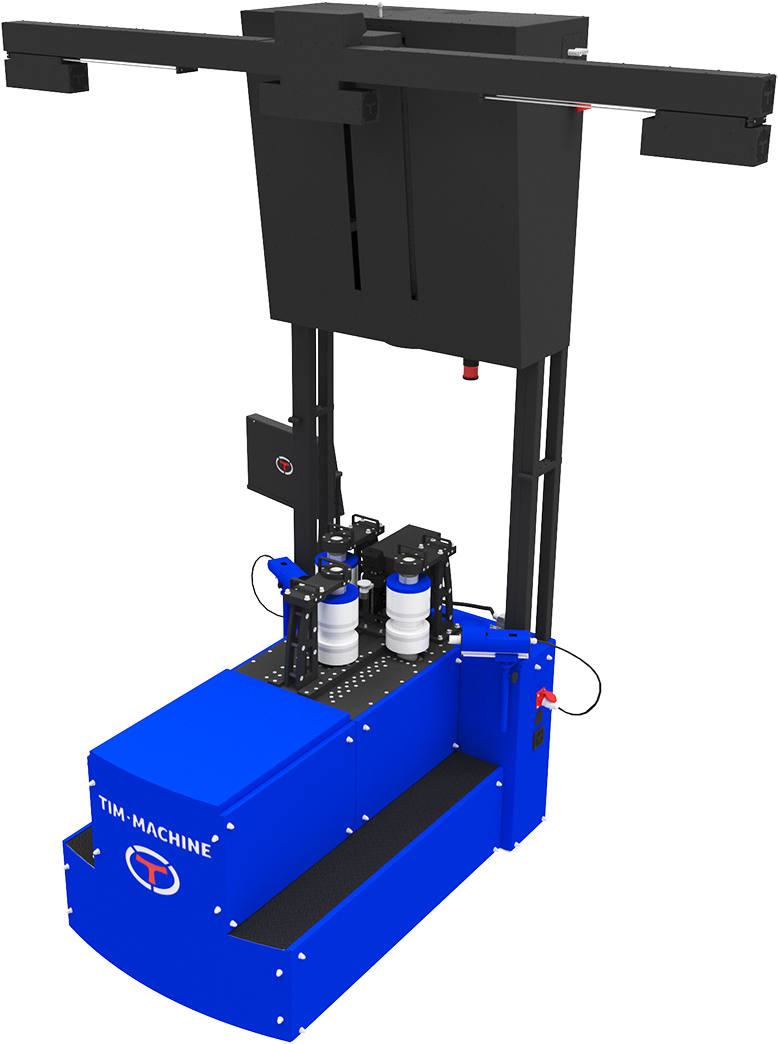
\includegraphics[height=9cm, width=6cm]{images/Masina_MODEL-M-CNC-3D.png}
     \captionof{figure}{TIM-MACHINE MODEL M-CNC-3D}
\end{center}
\vspace{0.5cm}

\newpage

\section{Поставка задатка}
Улазни податак на основу кога се одређује класа којој профил припада јесте слика која је генерисана од дубинске матрице коју даје 3D камера. Примјер такве слике је дат на следећој слици:
\vspace{0.5cm}
\begin{center}
    \centering 
    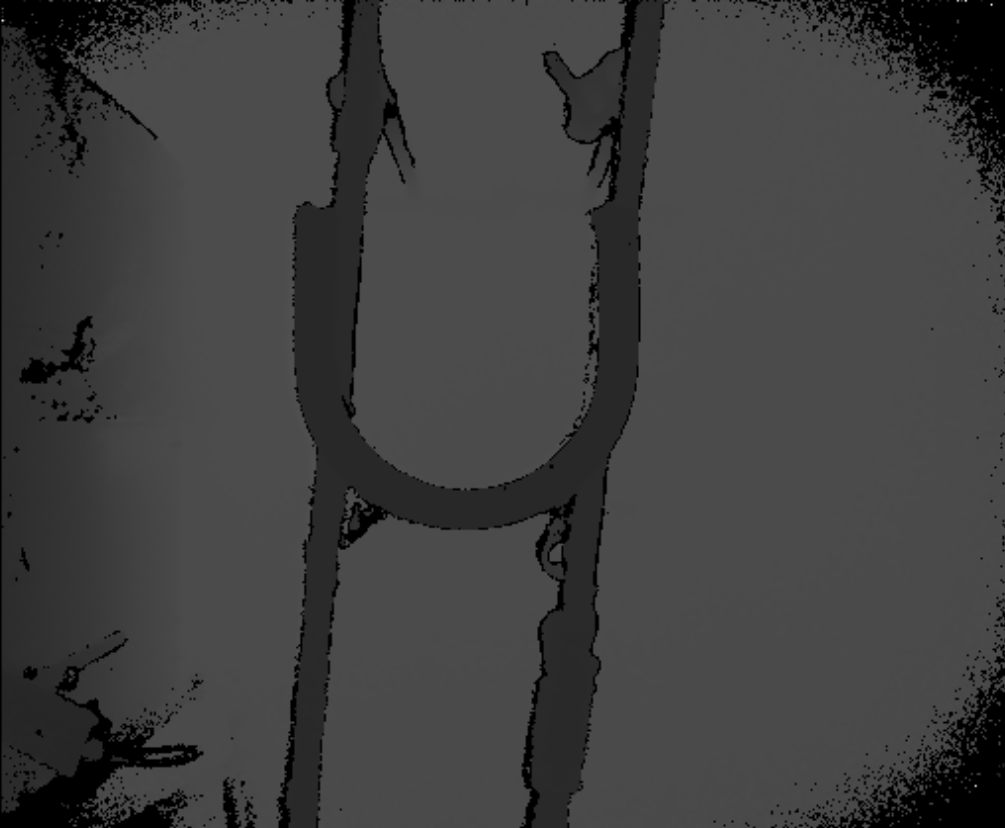
\includegraphics[height=6cm, width=8cm]{images/ulazna_slika.png}
     \captionof{figure}{Слика са 3D камере}
\end{center}
\vspace{0.5cm}
\indent\indentВидимо да се на слици налази промјерак савијеног профила који је постављен на двије хоризонталне шипке. Оно што је главни задатак јесте класификација профила са слике у једну од следећих класа:
\vspace{0.5cm}
\begin{center}
    \centering 
    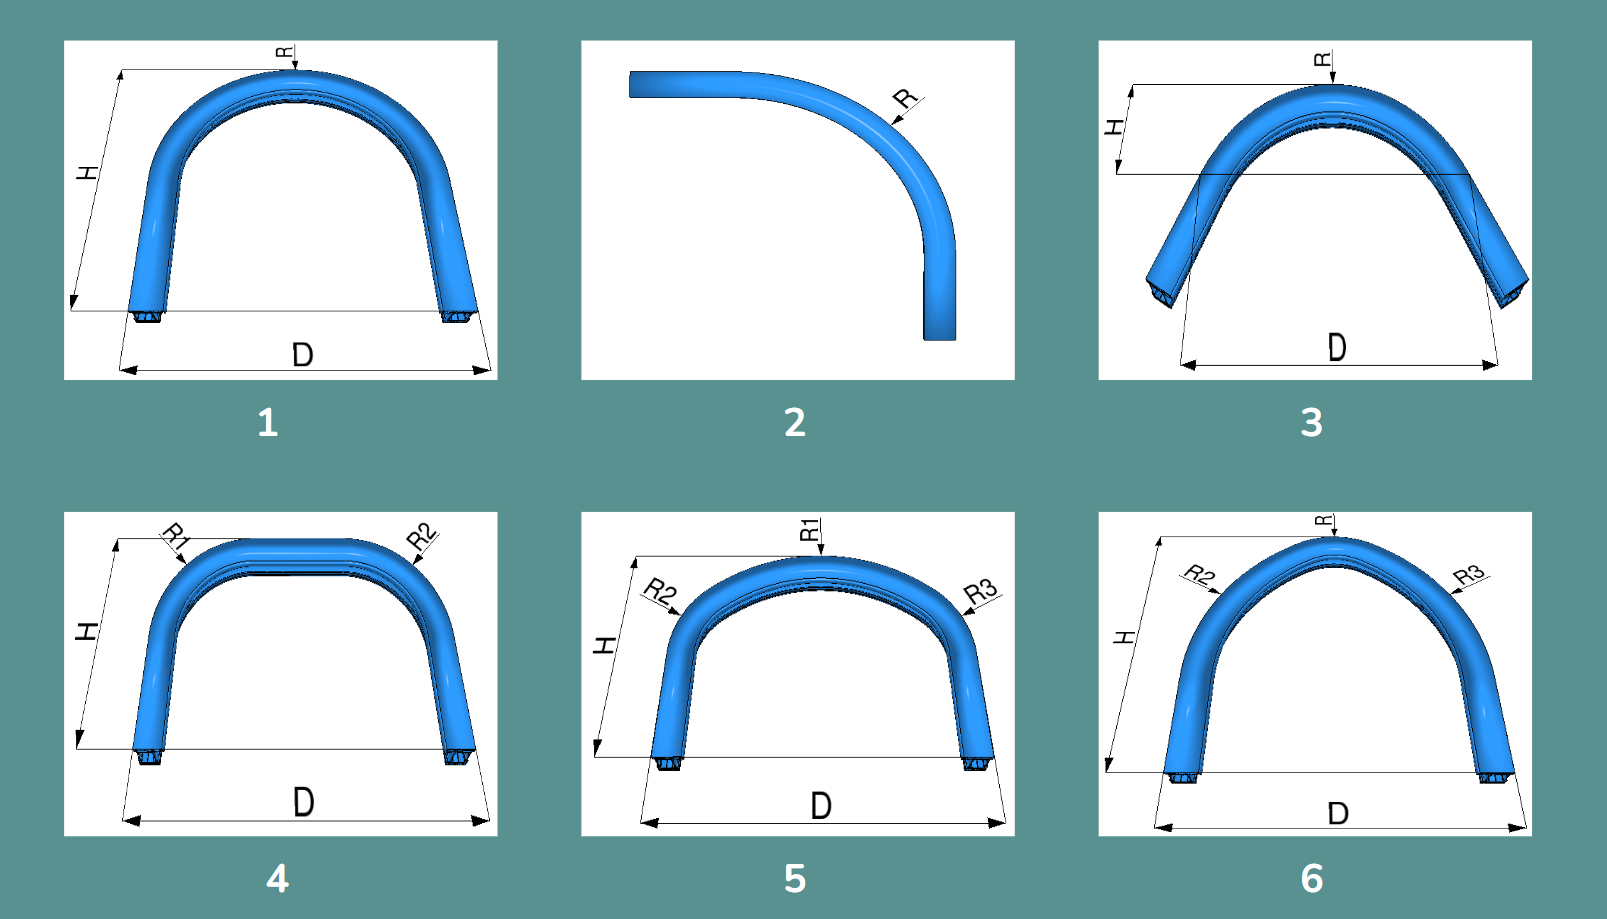
\includegraphics[height=9cm, width=15cm]{images/klase.png}
     \captionof{figure}{Класе профила}
\end{center}
\indent\indent Oчигледно је да примјерак профила са улазне слике припада класи означеној са 1 (правилан лук - заклапа $180^\circ$). Међутим, битно је напоменути да примјерци са претходне слике у пракси не морају бити идентични. На пример, равни дио на савијеним профилима не треба узимати у разматрање него само дио профила који представља лук, јер равни дио може у неким случајевима изостати, а у неким бити доста дужи, а да при томе угао лука остане исти.\\\\
\indent Карактеристике лукова сваке класе означене бројевима као на претходној слици су:
\begin{itemize}
  \item 1 - правилан лук (заклапа $180^\circ$)
  \item 2 - лук облика L (заклапа $90^\circ$)
  \item 3 - исјечак који заклапа угао мањи од $180^\circ$, при чему различито од $90^\circ$
  \item 4 - заклапа два угла по $90^\circ$
  \item 5 - састоји се из 3 исјечка сваки је мањи од $90^\circ$, али је угао на врху различит од углова са стране, док су углови са стране исти
  \item 6 - угао на врху је већи од $90^\circ$, а два са стране су мањи од $90^\circ$
\end{itemize}

\newpage

\section{Опис коришћене технологије}
За израду пројекта коришћене су следеће технологије:
\begin{itemize}
    \item 3D камера која даје дубинску матрицу за потребе обраде слике
    \item Већ савијени профили за тестирање
    \item C\# програмски језик
    \item Microsoft Visual Studio 2019 развојно окружење
    \item OpenCvSharp - OpenCv библиотека за обраду слике прилагођена развоју у C\#
    \item DepthBasics-WPF - започет пројекат који нуди основне могућности извлачења фрејмова са 3D камере и приказивање слике на основу дубинске матрице у оквиру WPF апликације израђене у C\#.
    \item Latex - описни језик за уређивање докуманата (коришћен  за израду писаног дијела пројектног задатка). При писању је коришћен онлајн уређивач који се назива \href{https://www.overleaf.com/project}{Overleaf} и пружа веома ефикасан и прилагођен интерфејс и брзину генерисања документа.
\end{itemize}

\newpage
\section{Структура пројекта}
Пројекат је рађен над већ постојећим пројектом који се назива DepthBasics-WPF и који садржи програм за повезивање на 3D камеру и извлачење података о дубини пиксела за сваки фрејм на снумку. Такође је урађен и једноставан графички интерфејс у коме се налази приказ обрађене дубинске матрице која се добија од камере. Структура датотека у пројекту је приказана на следећој слици:
\vspace{0.5cm}
\begin{center}
    \centering 
    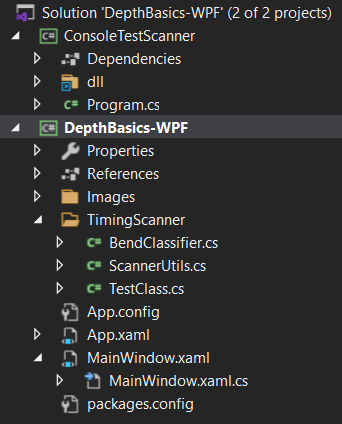
\includegraphics[height=10cm, width=8cm]{images/struktura.png}
     \captionof{figure}{Структура пројекта}
\end{center}
\vspace{0.5cm}
Над већ постојеће датотеке додати су: ConsoleTestScanner конзолна апликација за тестирање појединих дијелова кода у конзоли и датотеке (класе) у оквиру TimingScanner директоријума. Датотеке MainWindow.xaml и MainWindow.xaml.cs су надограђене за потребе развоја пројекта.

\newpage
\section{Имплементација и опис дијелова програма}
Да би класификација профила била обављена прецизно и успјешно, неоходно је правилно издвојити профил са фрејма који је извучен из снимка 3D камере. То је веома битан и сложен процес од којег нам касније зависи прецизност са којом можемо рећи да неки профил припада одређеној класи. Имплементација класификатора са све припремом података пролази кроз следеће фазе које ће у наставку бити детаљно образложене:
\begin{itemize}
    \item Постављање ограничења по дубини пиксела слике
    \item Отклањање шума на слици 
    \item Пребацивање сиве слике профила у црно-бијелу
    \item Проналазак највеће контуре на слици
    \item Корекција ротације профила
    \item Издвајање одбирака лука и њихово углачавање (усредњавање)
    \item Процес класификације
\end{itemize}
\indent\indent Битно је напоменути да све протходне фазе треба да се обављају редом како су написане. Покретањем програма отвара се прозор са приказом једног фрејма са снимка:
\vspace{0.5cm}
\begin{center}
    \centering 
    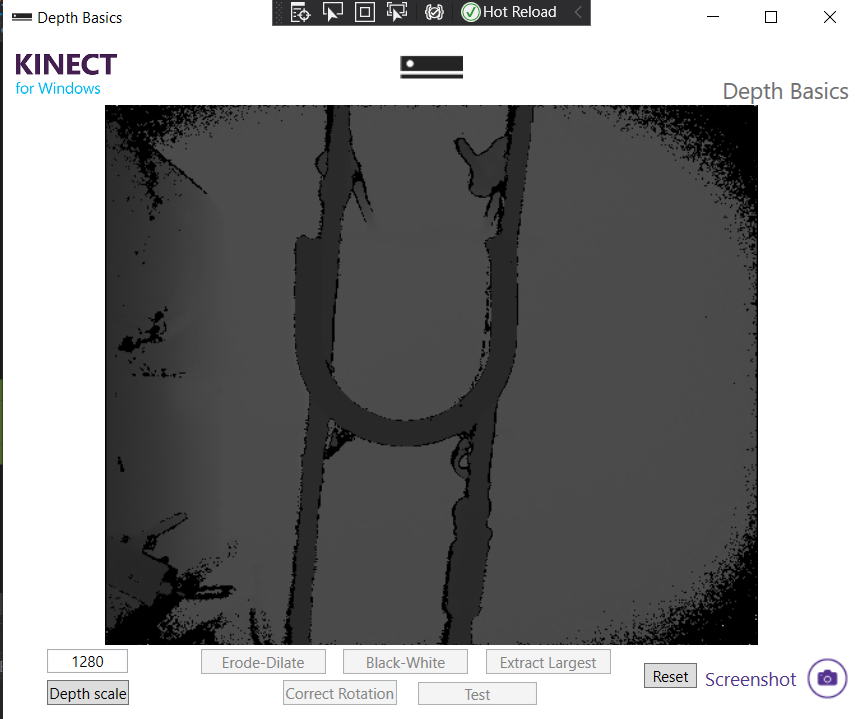
\includegraphics[height=10cm, width=12cm]{images/0_main_window.png}
     \captionof{figure}{MainWindow почетни приказ}
\end{center}
\vspace{0.5cm}
Дугмићи испод слике су додати на основни пројекат за потребе тестирања и демонстрације рада програма.

\subsection{Постављање ограничења по дубини пиксела слике}
Представља ограничавање дубине пиксела на неку вриједност. У нашем случају потребно је пронаћи профил по дубини, тако да се ништа испод профила не види. Уносом жељеног ограничења и кликом на дугме "Depth scale" добија се следећи приказ:
\vspace{0.5cm}
\begin{center}
    \centering 
    
\includegraphics[height=8cm, width=10cm]{images/2_depth.png}
     \captionof{figure}{Скалирање по дубини}
\end{center}
\vspace{0.5cm}
За претходну акцију задужена је функција:\\\\
\texttt{public static unsafe void ProcessDepthFrameDataFromCsv(ushort[] depthFrameData, byte[] depthPixels, ushort minDepth, ushort maxDepth)}\\\\
из TimingScanner.ScannerUtils класе.\\\\
Функција не враћа ништа, а као параметре има:
\begin{itemize}
    \item \texttt{ushort[] depthFrameData} - низ неозначених 16-битних цјелобројних вриједности које представљају дубине сваког пиксела
    \item \texttt{byte[] depthPixels} - низ 8-битних цјелобројних вриједности у који се пакују вриједности првог аргумента конвертоване у 8-битне и скалиране по дубини
    \item \texttt{ushort minDepth} - доње ограничење на дубину
    \item \texttt{ushort maxDepth} - горње ограничење на дубину
\end{itemize}
Треба напоменути да су фрејмови учитани из .csv фајла због немогућности свакодневног приступа камери и снимању профила уживо.

\subsection{Отклањање шума на слици}
Односи се на занемаривање ситних дијелова тј. пиксела који нису дијелови профила, а који су "ухваћени" на истој дубини као профил. Такође помаже при углачавању ивица профила. Резултат отклањања шума са претходне слике је приказан на следећој слици:
\vspace{0.5cm}
\begin{center}
    \centering 
    
\includegraphics[height=8cm, width=10cm]{images/3_erode_dilate.png}
     \captionof{figure}{Отклоњен шум}
\end{center}
\vspace{0.5cm}
За претходну акцију задужена је функција:
\begin{center}
\texttt{public static Mat ErodeDilateImage(Mat srcImg)}
\end{center}
из TimingScanner.ScannerUtils класе.\\\\
Функција враћа матрицу слике типа Mat са отклоњеним шумом, а као параметар има:
\begin{itemize}
    \item \texttt{Mat srcImg} - матрица слике типа Mat скалирана по дубини
\end{itemize}
Унутар ове функције позивају се функције \href{https://shimat.github.io/opencvsharp\_docs/html/6bfd2ddd-6fb6-ce1e-a07c-28317b1e8bc6.htm}{Erode} и \href{https://shimat.github.io/opencvsharp_docs/html/c5e6c07a-feae-9588-e690-703911dd81dc.htm}{Dilate} из OpenCvSharp библиотеке и то по редослиједу Erode-Dilate-Erode, са елиптичким кернелима величина 4х4, 7х7, 3х3 редом.

\newpage
\subsection{Пребацивање сиве слике профила у црно-бијелу}
Односи се на пребацивање свих пиксела који нису црни (оних различитих од 0) у потпуно бијелу боју (вриједност 255). Од претходне слике добија се следећа:
\vspace{0.5cm}
\begin{center}
    \centering 
    
\includegraphics[height=8cm, width=10cm]{images/4_black_white.png}
     \captionof{figure}{Црно-бијела слика}
\end{center}
\vspace{0.5cm}
За претходну акцију задужена је функција:
\begin{center}
\texttt{public static Mat ToBlackWhiteImage(Mat srcImg)}
\end{center}
из TimingScanner.ScannerUtils класе.\\\\
Функција враћа матрицу слике типа Mat са вриједностима 0 или 255, а као параметар има:
\begin{itemize}
    \item \texttt{Mat srcImg} - матрица слике типа Mat са отклоњеним шумом
\end{itemize}

\newpage
\subsection{Проналазак највеће контуре на слици}
Претпоставка је да је, по диманзијама, профил највећа контура на слици. С обзиром да је то једина контура од интереса и да на слици могу постојати и неке друге, мање контуре као што је случај на претходној слици, потребно је издвојити само контуру профила тако да се добије следећи приказ:
\vspace{0.5cm}
\begin{center}
    \centering 
    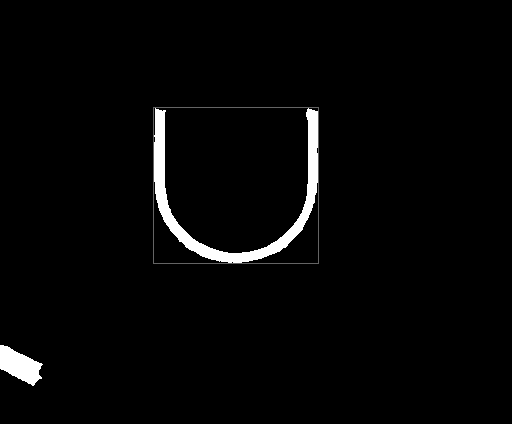
\includegraphics[height=8cm, width=10cm]{images/5_find_largest.png}
     \captionof{figure}{Пронађена највећа контура на слици}
\end{center}
\vspace{0.5cm}
\vspace{0.5cm}
\begin{center}
    \centering 
    
\includegraphics[height=4.5cm, width=5cm]{images/6_extract_largest.png}
     \captionof{figure}{Издвојена највећа контура (профил) са слике}
\end{center}
\vspace{0.5cm}
За претходну акцију задужена је функција:
\begin{center}
\texttt{\textbf{public static Mat ExtractLargestContour(Mat srcImg, bool onlyFind)}}
\end{center}
из TimingScanner.ScannerUtils класе.\\\\
Функција враћа матрицу слике типа Mat са издвојеном само највећом контуром на слици, а као параметре има:
\begin{itemize}
    \item \texttt{Mat srcImg} - матрица слике типа Mat (црно-бијела)
    \item \texttt{bool onlyFind} - логичка вриједност која ако је true значи да функција враћа матрицу истих димензија као улазна слика на којој је пронађена највећа контура уоквирена у четвероугао. Ако је false функција враћа издвојену навећу контуру тј. матрицу димензија највеће контуре.
\end{itemize}

\subsection{Корекција ротације профила}
У претходним случајевима имали смо правилно окренут профил крацима ка горе. Међутим, то не мора увијек бити тако. На примјер, профил може бити окренут и као на следећој слици:
\vspace{0.5cm}
\begin{center}
    \centering 
    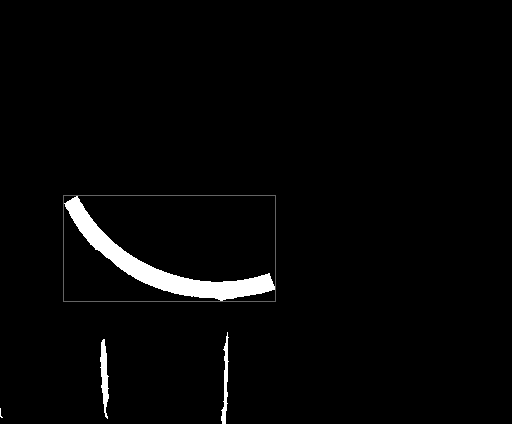
\includegraphics[height=8cm, width=10cm]{images/7_section_bend.png}
     \captionof{figure}{Профил прије ротације}
\end{center}
\vspace{0.5cm}
Након издвајања и ротације, добија се профил који је постављен као на следећој слици:
\vspace{0.5cm}
\begin{center}
    \centering 
    
\includegraphics[height=1.5cm, width=5cm]{images/8_correct_rotation.png}
     \captionof{figure}{Профил послије ротације}
\end{center}
\vspace{0.5cm}
За претходну акцију задужена је функција:
\begin{center}
\texttt{public static Mat correctRotation(Mat srcImg)}
\end{center}
из TimingScanner.ScannerUtils класе.\\\\
Функција враћа матрицу слике типа Mat са ротираном улазном сликом тако да је на њој профил окренут крацима ка горе, а као параметар има:
\begin{itemize}
    \item \texttt{Mat srcImg} - матрица слике типа Mat са издвојеним профилом
\end{itemize}
Логика за корекцију ротације је следећа:\\
Иницијализујемо два низа за по 90 елемената. Затим улазну слику кроз 90 итерација ротирамо за по $1^\circ$. У свакој итерацији новоротирана слика се подијели на два дијела, прво горњи и доњи, доњи се флипује и одузима се елемент по елемент од горњег, и онда се те вриједности разлика сумирају и стављају у први низ. У истој итерацији се исто одради и за лијеву и десну половину слике, а коначна вриједност разлике се убаци у други низ. Након 90 итерација имамо 2 низа и из оба извучемо минимум. Затим упоредимо који од та два минимума је мањи и из ког низа је тај минимум. Затим \textbf{улазну слику} са почетка ротирамо за вриједност индекса + 1 на којем је мањи минимум у свом низу. Ако је тај минимум из првог низа, на последње ротираној слици биће профил који је окренут крацима ка лијево или ка десно. Ако је из другог низа, профил је окренут крацима ка горе или ка доле. Након тога се детектује да ли је профил окренут крацима ка горе или ка доле за случај горе-доле положаја, односнода ли је окренут крацима ка лијево или десно за случај лијево-десно положаја профила. Након тога се слика лако ротира како би излазна слика била слика профила са крацима окренутим ка горе.\\
Унутар горе поменуте функције користе се и још неке функције битне за корекцију ротације које су имплементиране у оквиру овог пројекта, а то су:\\\\
\texttt{public static Mat MatRotate(Mat src, float angle)},\\
\texttt{public static Mat correctHorizontalBend(Mat srcImg)} и \\
\texttt{public static Mat correctVerticalBend(Mat srcImg)}\\\\
све у оквиру TimingScanner.ScannerUtils класе

\newpage
\subsection{Издвајање одбирака лука и њихово углачавање (усредњавање)}
Да бисмо издвојили одбирке лука потребно је окренути лук крацима ка горе и координатни систем се поставља у доњи лијеви угао издвојене слике:
\vspace{0.5cm}
\begin{center}
    \centering 
    
\includegraphics[height=4.5cm, width=5cm]{images/9_za_odbirke.png}
     \captionof{figure}{Профил припремљен за узимање одбирака лука}
\end{center}
\vspace{0.5cm}
С обзиром да лук у овом положају има симетричну лијеву и десну страну, разматраћемо само једну (лијеву) страну лука:
\vspace{0.5cm}
\begin{center}
    \centering 
    
\includegraphics[height=4.5cm, width=2.5cm]{images/10_za_odbirke_pola.png}
     \captionof{figure}{Једна страна лука за узимање одбирака лука}
\end{center}
\vspace{0.5cm}
Ширина претходне слике је 100 пиксела и толико имамо одбирака. Одбирци по х-оси су цјелобројне вриједности од 1 до 100 и има их 100, а по у-оси су израчунате вриједности на основу облика лука полазећи с лијеве стране горње слике ка десно. Има их такође 100 и цјелобројне су вриједности:
\vspace{0.5cm}
\begin{center}
    \centering 
    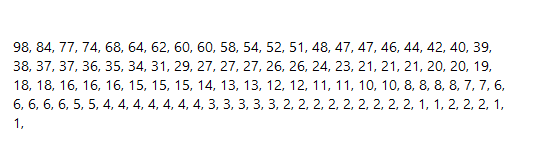
\includegraphics[height=3cm, width=9cm]{images/11_odbirci.png}
     \captionof{figure}{Одбирци лука по у-оси}
\end{center}
\vspace{0.5cm}
Претходни одбирци се добијају из функције: 
\begin{center}
\texttt{public static int[] getArrayY(Mat scaledImg)}
\end{center}
из TimingScanner.ScannerUtils класе.\\\\
Функција враћа низ цјелобројних вриједности одбирака по у-оси, а као параметар има:
\begin{itemize}
    \item \texttt{Mat scaledImg} - матрица слике типа Mat која представља половину лука
\end{itemize}

Ако погледамо претходне одбирке, видимо да се неки дијелови лука детектују као равни због репрезентације у цјелобројним вриједностима. Због тога је претходни низ потребно пребацити у низ децималних вриједности које ће прецизније да описују закривљења лука тј. потребно је углачати (усредњити) вриједности одбирака лука. да би смо то постигли користи се техника \textbf{Average Pooling} којом се са 1D филтером жељене величине (непаран број) крећемо кроз низ са кораком 1 и сваку вриједност која се нађе у "средини" филтера мијењамо са просјечном вриједношћу свих околних вриједности које у том моменту захвата филтер.\\\\
Претходни одбирци се добијају из функције: 
\begin{center}
\texttt{public static float[] AveragePoolingSmooth1D(float[] srcArr, int filterSize, int numIter = 1)}
\end{center}
из TimingScanner.ScannerUtils класе.\\\\
Функција враћа низ децималних вриједности одбирака по у-оси (низ је исте дужине као улазни), а као параметре има:
\begin{itemize}
    \item \texttt{float[] srcArr} - низ децималних вриједности које требају бити усредњене
    \item \texttt{int filterSize} - величина 1D филтера којим пролазимо кроз низ
    \item \texttt{int numIter = 1} - број пута колико желимо да одрадимо усредњавање улазног низа са одабраном величином филтера (подразумјевано је 1 итерација)
\end{itemize}
Ако горе приказане цјелобројне одбирке пребацимо у низ децималних вриједности, и такав низ прослиједимо претходно наведеној функцији добија се следећи низ:
\vspace{0.5cm}
\begin{center}
    \centering 
    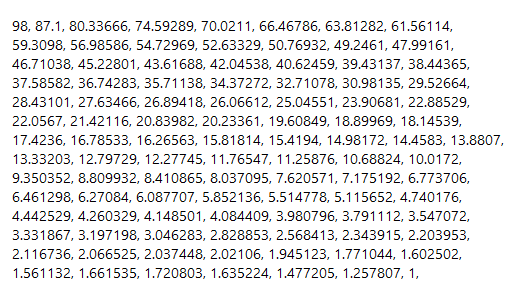
\includegraphics[height=5cm, width=10cm]{images/12_odbirci_average.png}
     \captionof{figure}{Усредњене вриједности одбирака лука}
\end{center}
\vspace{0.5cm}
Прва и последња вриједност у низу остају непромјењенем како не бисмо губили информацију одакле лук почиње и гдје се тачно завршава. Претходно приказане одбирке добили смо тако што смо прво одрадили један пролазак коришћењем филтера дужине 5, а затим добијени низ још једном усредњавамо филтером дужине 3.\\
Оно што је представља проблем јесу профили који имају краке са незакривљеним продужецима који нису паралелни, као што је то приказано на следећој слици:
\vspace{0.5cm}
\begin{center}
    \centering 
    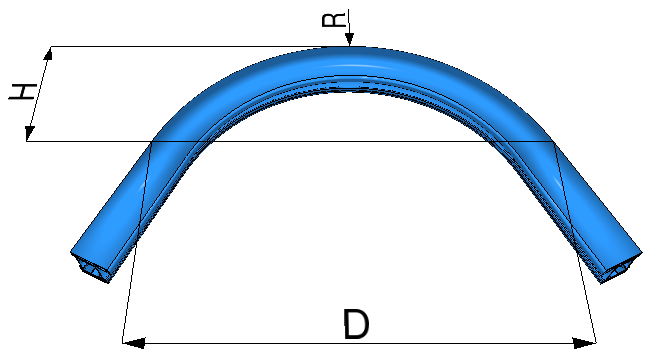
\includegraphics[height=5cm, width=7cm]{images/klasa3.jpg}
     \captionof{figure}{Профил са непаралелним равним продужецима}
\end{center}
\vspace{0.5cm}
Са слике видимо да ће, када се профил окрене крацима ка горе, одбирци захватити и раван дио који не припада луку, што није добро јер у обзир треба узети само лук. Проблем је узет у обзир кроз класификацију и то представља привремено рјешење док се не развије алгоритам за детекцију равног дијела профила.


\newpage
\section{Процес класификације}
Функције за класификацију смјештене су у TimingScanner.BendClassifier класи. Класификација се одвија методом елиминације. За потребе једноставнијег означавања, класе лукова су означене бројевима на следећи начин:
\vspace{0.5cm}
\begin{center}
    \centering 
    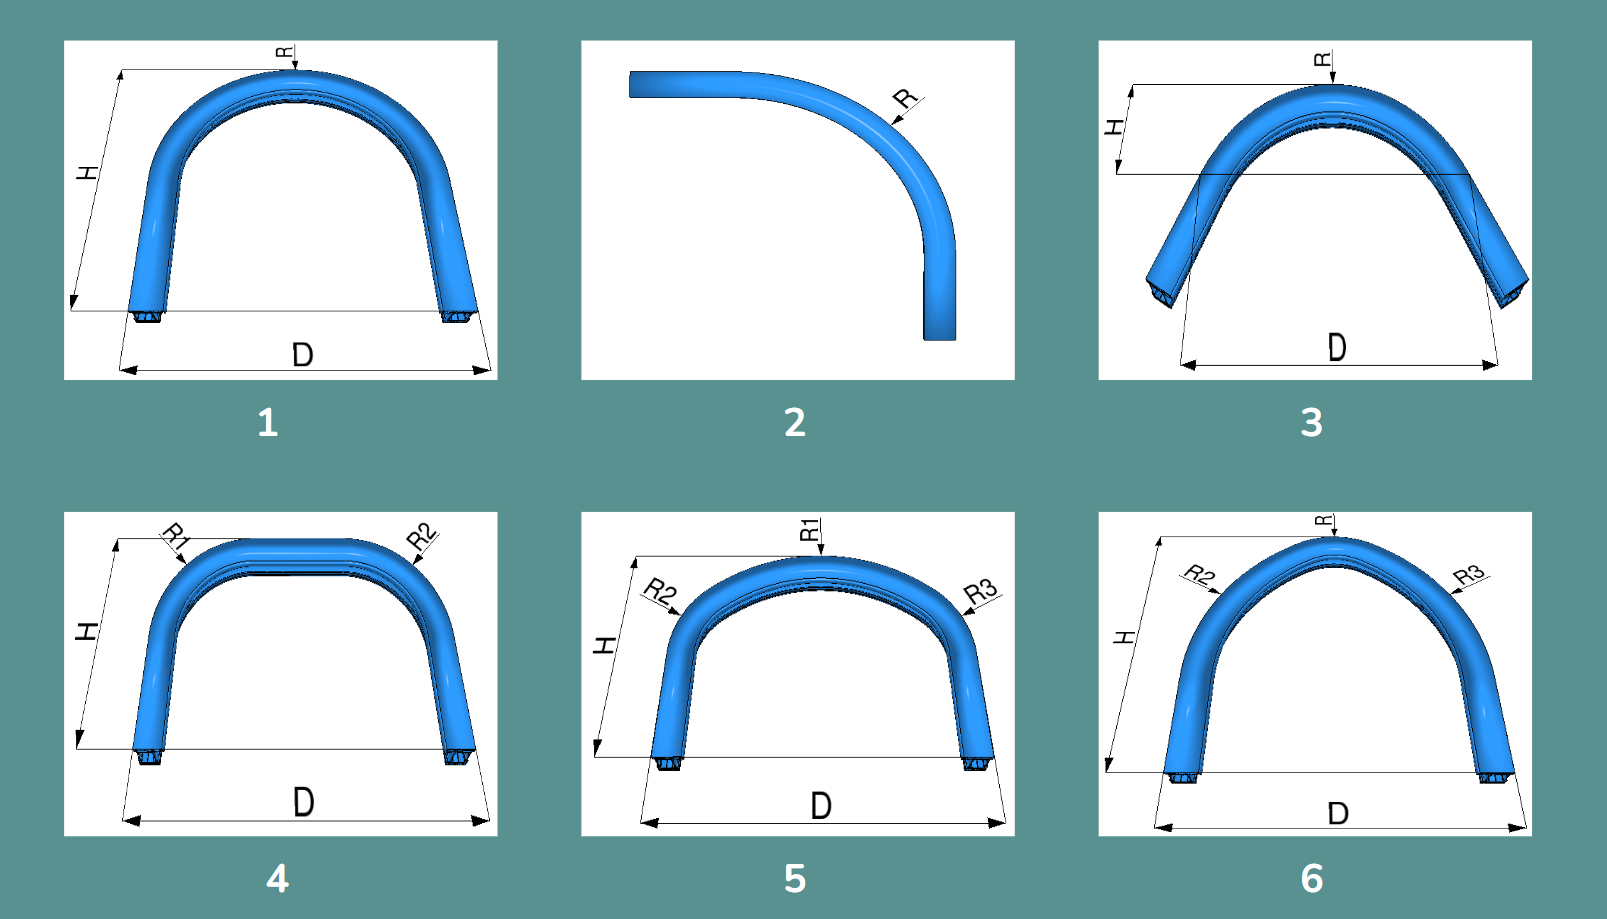
\includegraphics[height=9cm, width=15cm]{images/klase.png}
     \captionof{figure}{Класе профила}
\end{center}
\vspace{0.5cm}
Лукови се класификују следећим редослиједом, методом елиминације, тако да ако нпр. прође провјера за класу 1, даље се не провјерава, а ако не, тада се иде даље с провјером, с тим да је класа 1 одбачена и не може више бити детектована. Елиминација се обавља следећим редослиједом:
\begin{itemize}
    \item Провјера за класу 1 (правилан лук - заклапа $180^\circ$)
    \item Провјера за класу 2 (L лук - заклапа $90^\circ$)
    \item Провјера за класу 4 (састоји се од два L лука и заклапа $180^\circ$)
    \item Провјера за класу 6 (вертикална елипса)
    \item Провјера за класу 3.1 (исјечак без равног дијела)
    \item Провјера за класе 3 (исјечак са равним дијелом) и 5 (хоризонтална елипса)
\end{itemize}

\subsection{Провјера за класу 1 (правилан лук - заклапа $180^\circ$)}
\vspace{0.5cm}
\begin{center}
    \centering 
    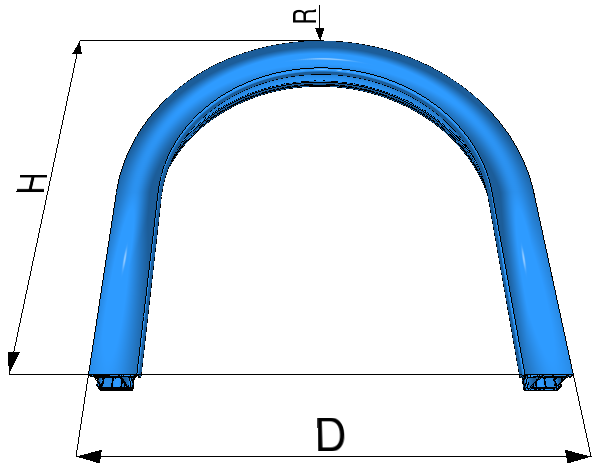
\includegraphics[height=4cm, width=6cm]{images/klasa1.jpg}
     \captionof{figure}{Класа 1}
\end{center}
\vspace{0.5cm}
За провјеру је задужена функција:
\begin{center}
\texttt{public static string detectBend1(Mat srcImg, float err1, float err2)}
\end{center}
из TimingScanner.bendClassifier класе.\\\\
Функција враћа стринг у коме су резултати провјере, а као параметре има:
\begin{itemize}
    \item \texttt{Mat srcImg} - улазна слика профила издвојена и ротирана тако да су краци профила окренути ка горе 
    \item \texttt{float err1} - дозвољено одступање 1
    \item \texttt{float err2} - дозвољено одступање 2
\end{itemize}
Унутар те функције се узима лијева половина улазне слике и позива се функција:
\begin{center}
\texttt{public static string detectBend1FromHalf(Mat srcImg, float err1, float err2)}
\end{center}
из TimingScanner.bendClassifier класе, гдје је \texttt{srcImg} сада лијева половина улазне слике у функцију \texttt{detectBend1}. Све провјере се врше унутар функције \texttt{detectbend1FromHalf}.\\\\
Провјера се врши у 3 фазе и све фазе морају дати позитиван резултат да би се профил смјестио у класу 1. Претпостављамо да лук припада 1. класи. Тада се врше следеће провјере:\\
а) Узима се низ одбирака по у-оси са лијеве стране и вриједност првог одбирка се пореди са ширином половине профила која је по претпоставци полупречник круга. Дозвољено одступање је једнако err1 аргументу. Ако апсолутан разлика поређених вриједности не одступа више од дозвољене вриједности, тада је услов задовољен. \vspace{0.5cm}
\begin{center}
    \centering 
    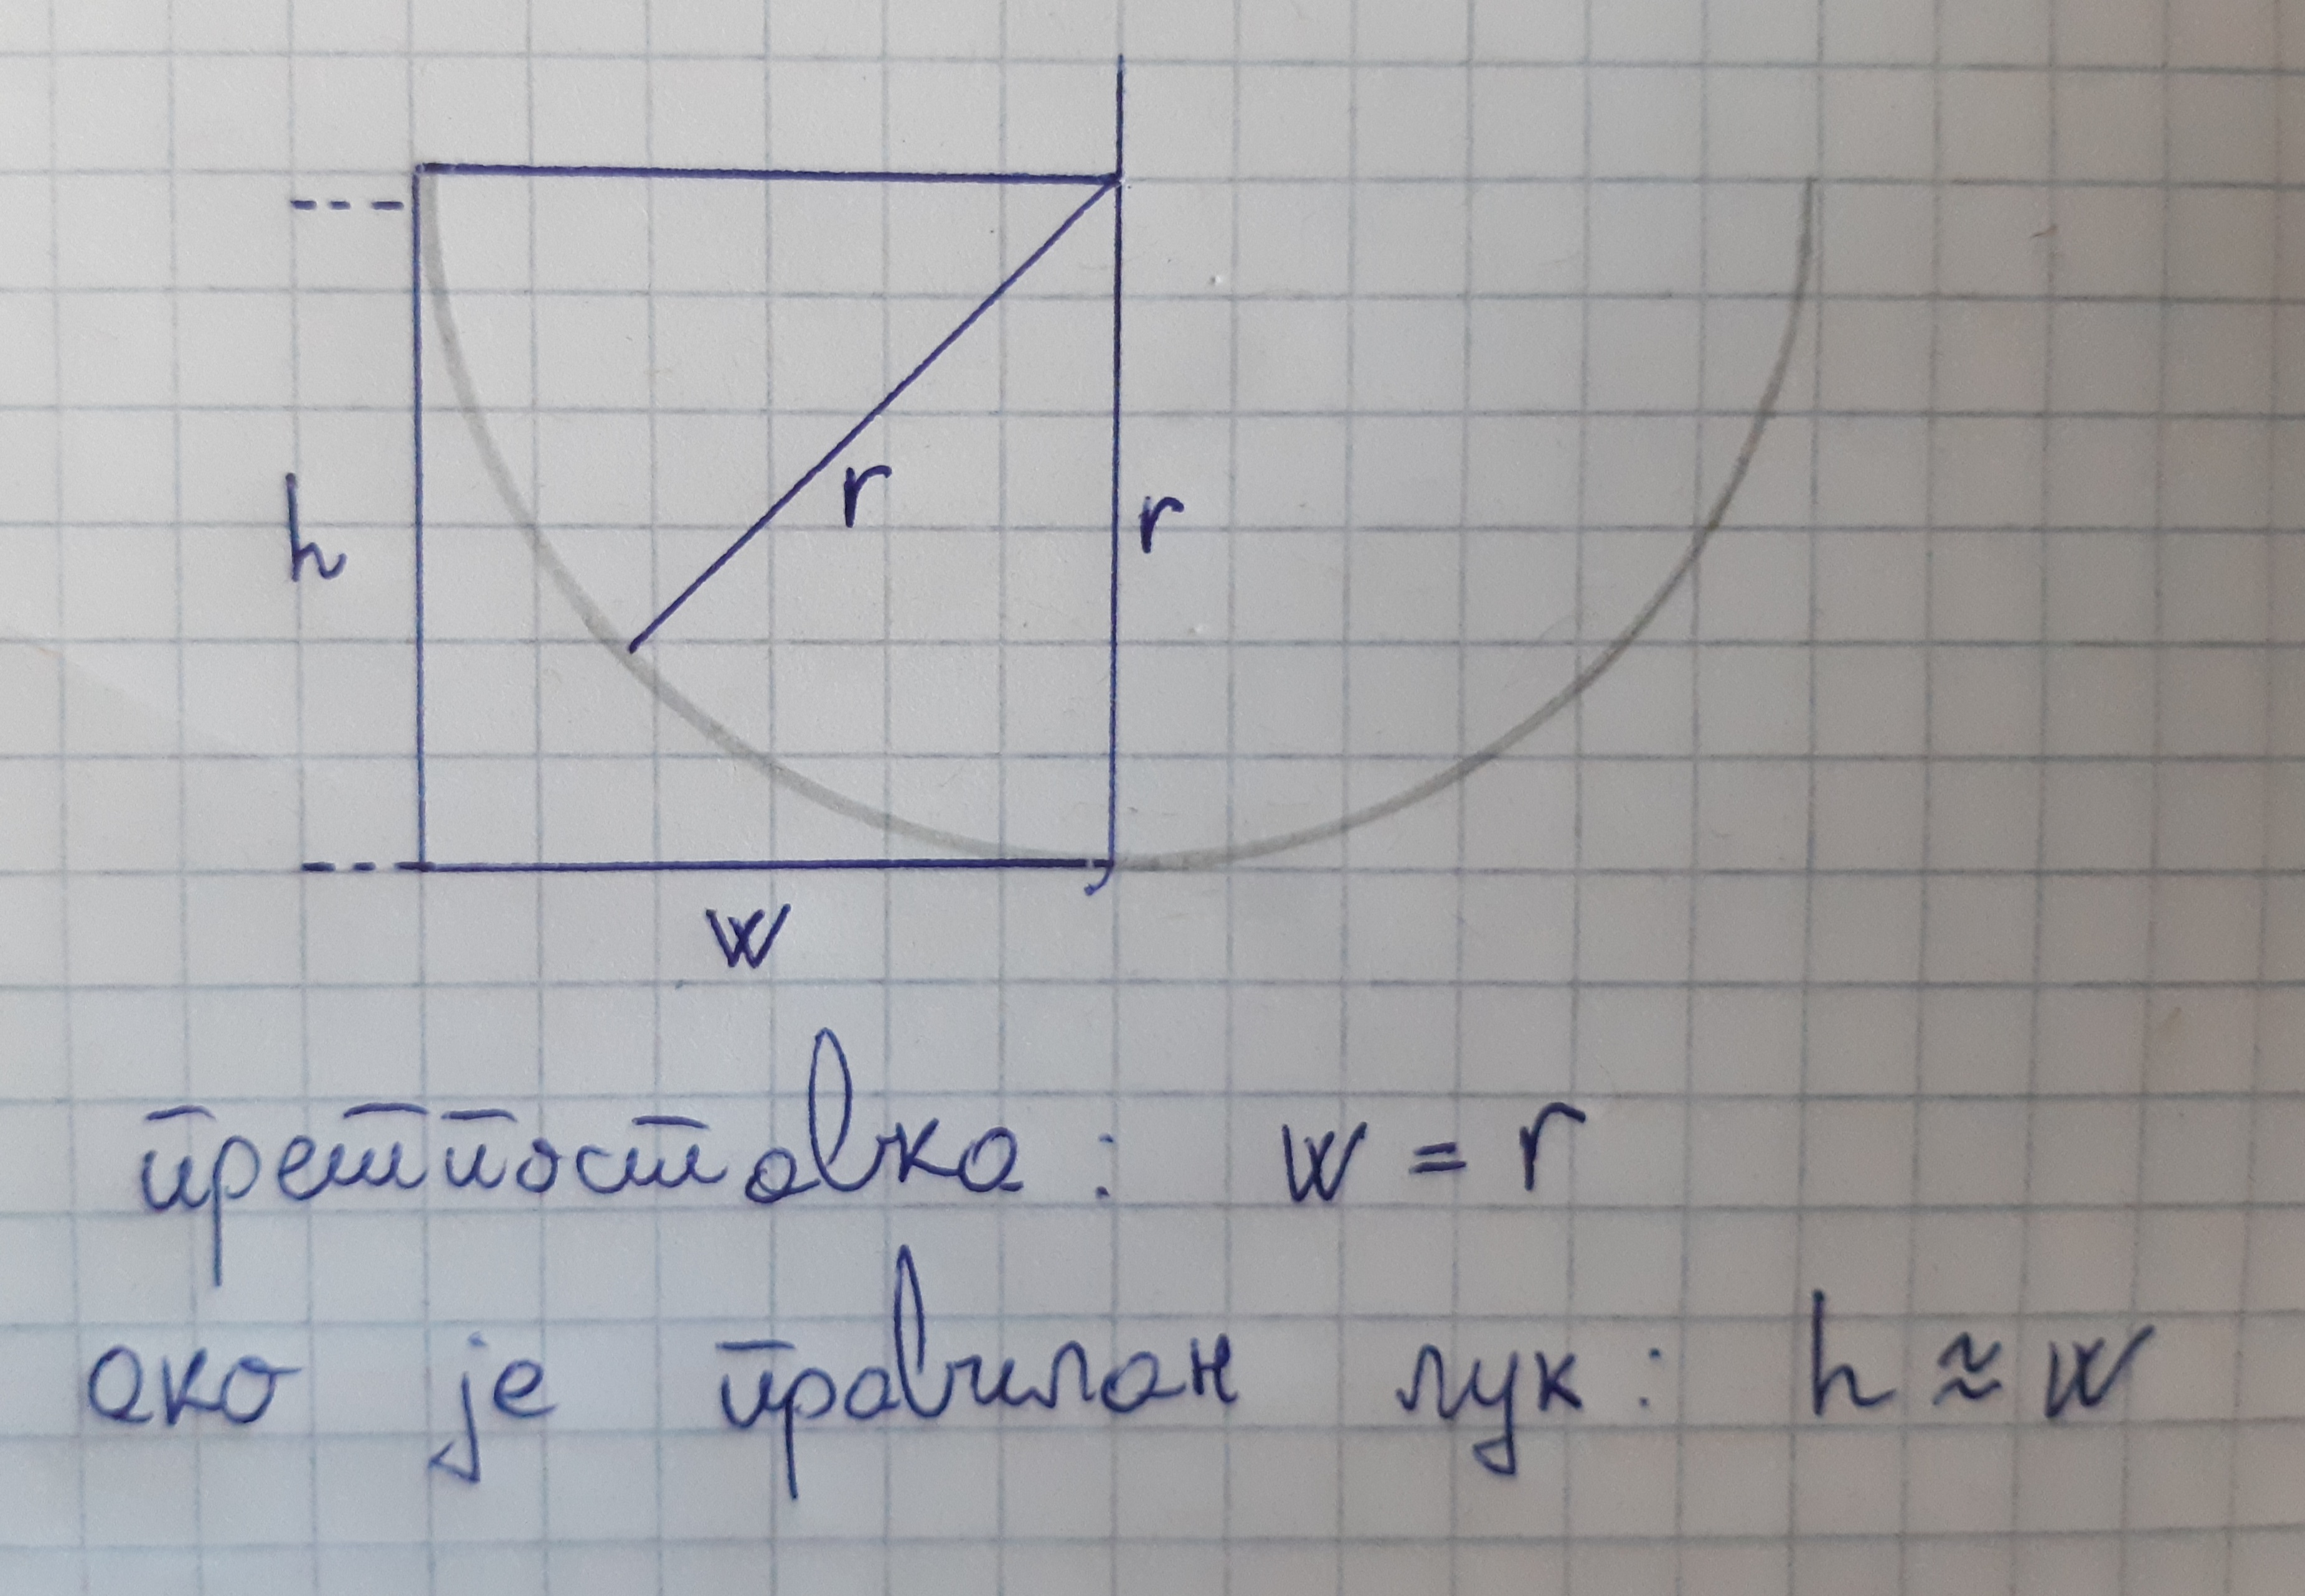
\includegraphics[height=5cm, width=7cm]{images/detect1.jpg}
     \captionof{figure}{Услов а)}
\end{center}
\vspace{0.5cm}
б) Такође узимамо да је полупречник једнак половини ширине профила тј. ширини слике која се прослијеђује као аргумент функцији \texttt{detectbend1FromHalf}. Вршимо усредњавање низа одбирака и провјеравамо да ли су све тачке на кружници са поменутим полупречником. Одступање у овом случају је 5\%. Ако се детектује секвенца већа дужа од 3 одбирка за редом која одступају преко дозвољене вриједности, тада овај услов није задовољен.\\
в) Као у претходном случају, потребан нам је низ усредњених вриједности одбирака. У овој провјери имамо једну тачку од значаја ако је лук правилан. Приказана је на следећој слици:
\vspace{0.5cm}
\begin{center}
    \centering 
    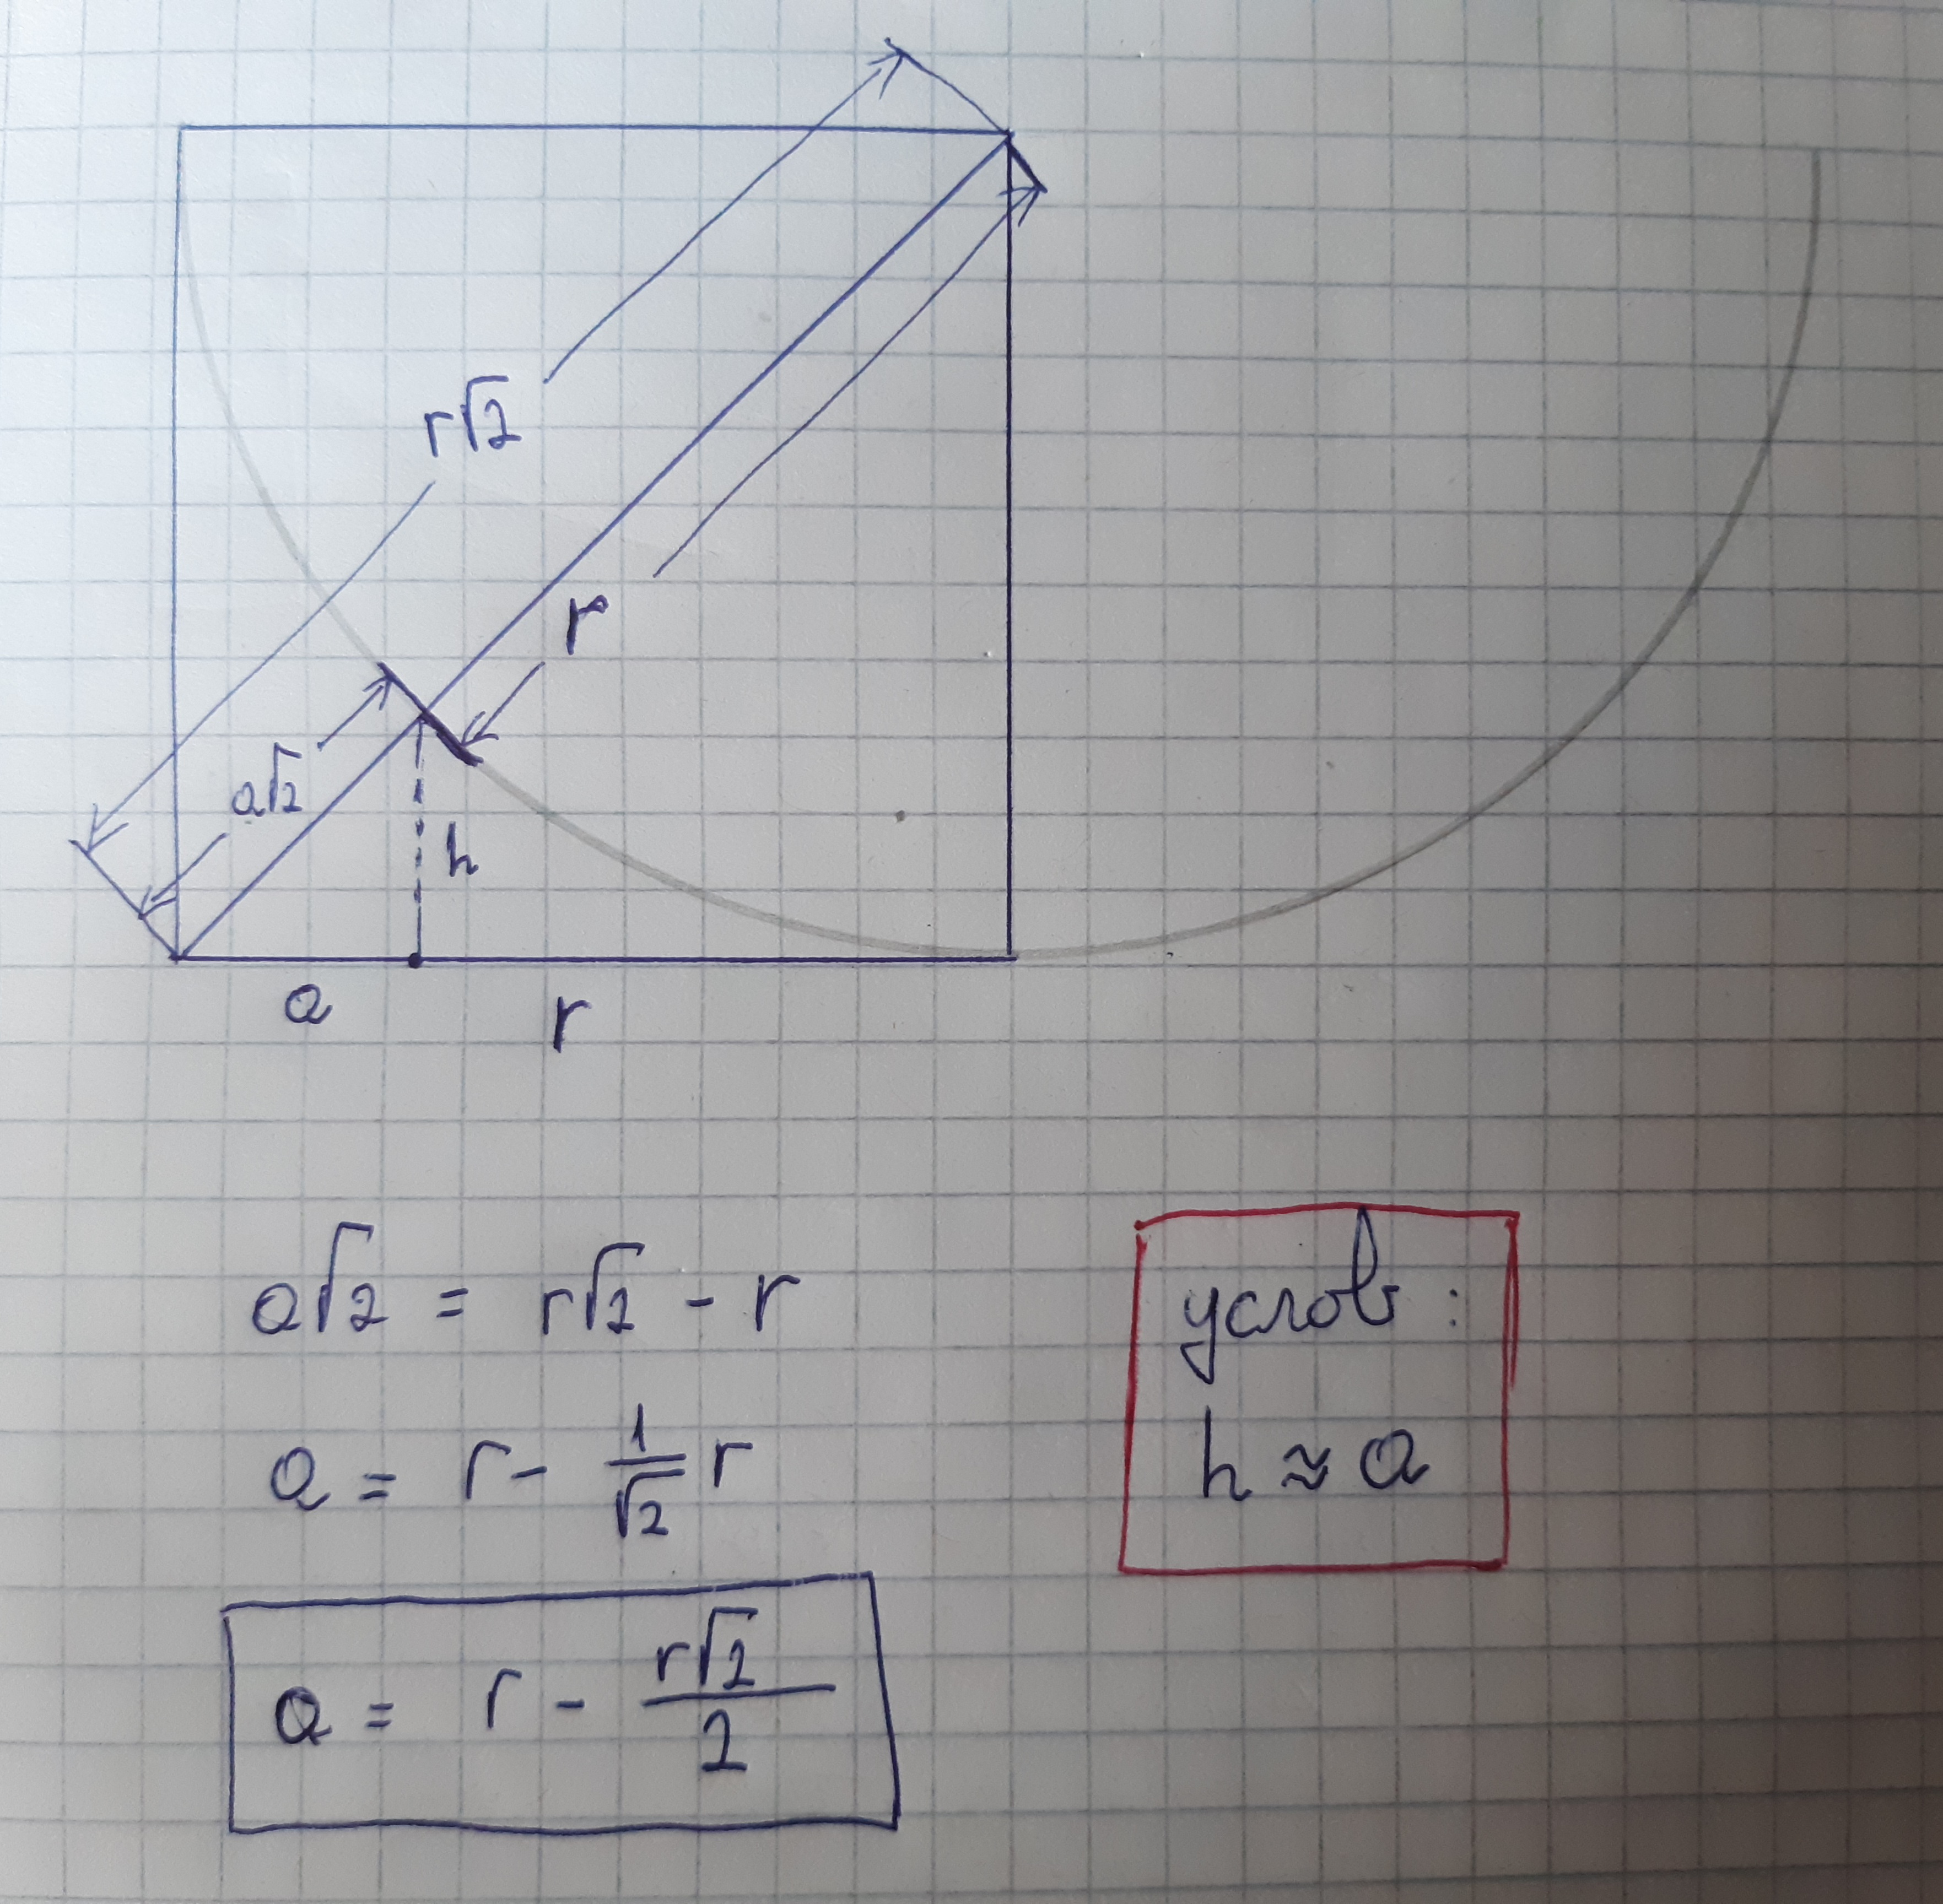
\includegraphics[height=9cm, width=9cm]{images/detect2.jpg}
     \captionof{figure}{Класа 1}
\end{center}
\vspace{0.5cm}

Одступање у овом случају је err2. Ако је одступање веће од дозвољеног, услов није задовољен.

\subsection{Провјера за класу 2 (L лук - заклапа $90^\circ$)}
\vspace{0.5cm}
\begin{center}
    \centering 
    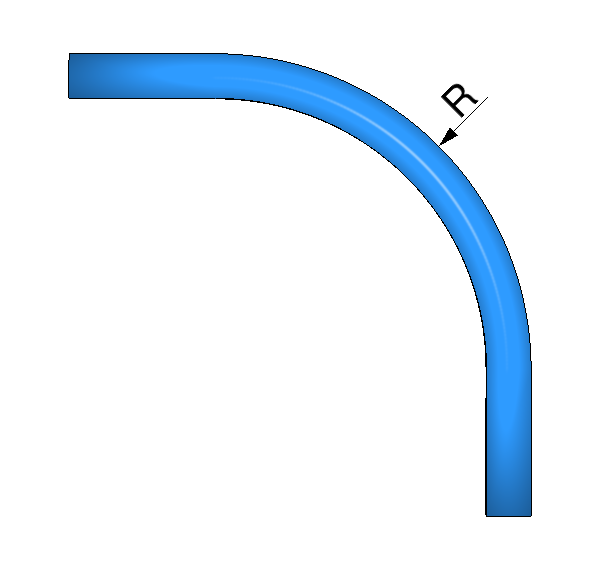
\includegraphics[height=5cm, width=7cm]{images/klasa2.jpg}
     \captionof{figure}{Услов в)}
\end{center}
\vspace{0.5cm}
За провјеру је задужена функција:
\begin{center}
\texttt{public static string detectBend2(Mat srcImg)}
\end{center}
из TimingScanner.bendClassifier класе.\\\\
Функција враћа стринг у коме су резултати провјере, а као параметap има:
\begin{itemize}
    \item \texttt{Mat srcImg} - улазна слика профила издвојена и ротирана тако да су краци профила окренути ка горе 
\end{itemize}
Унутар те функције се улазна слика ротира за $45^\circ$ супротно казаљци на сату, тј ради се следеће (претпоставка је ра је улазна слика слика лијево):
\vspace{0.5cm}
\begin{center}
    \centering 
    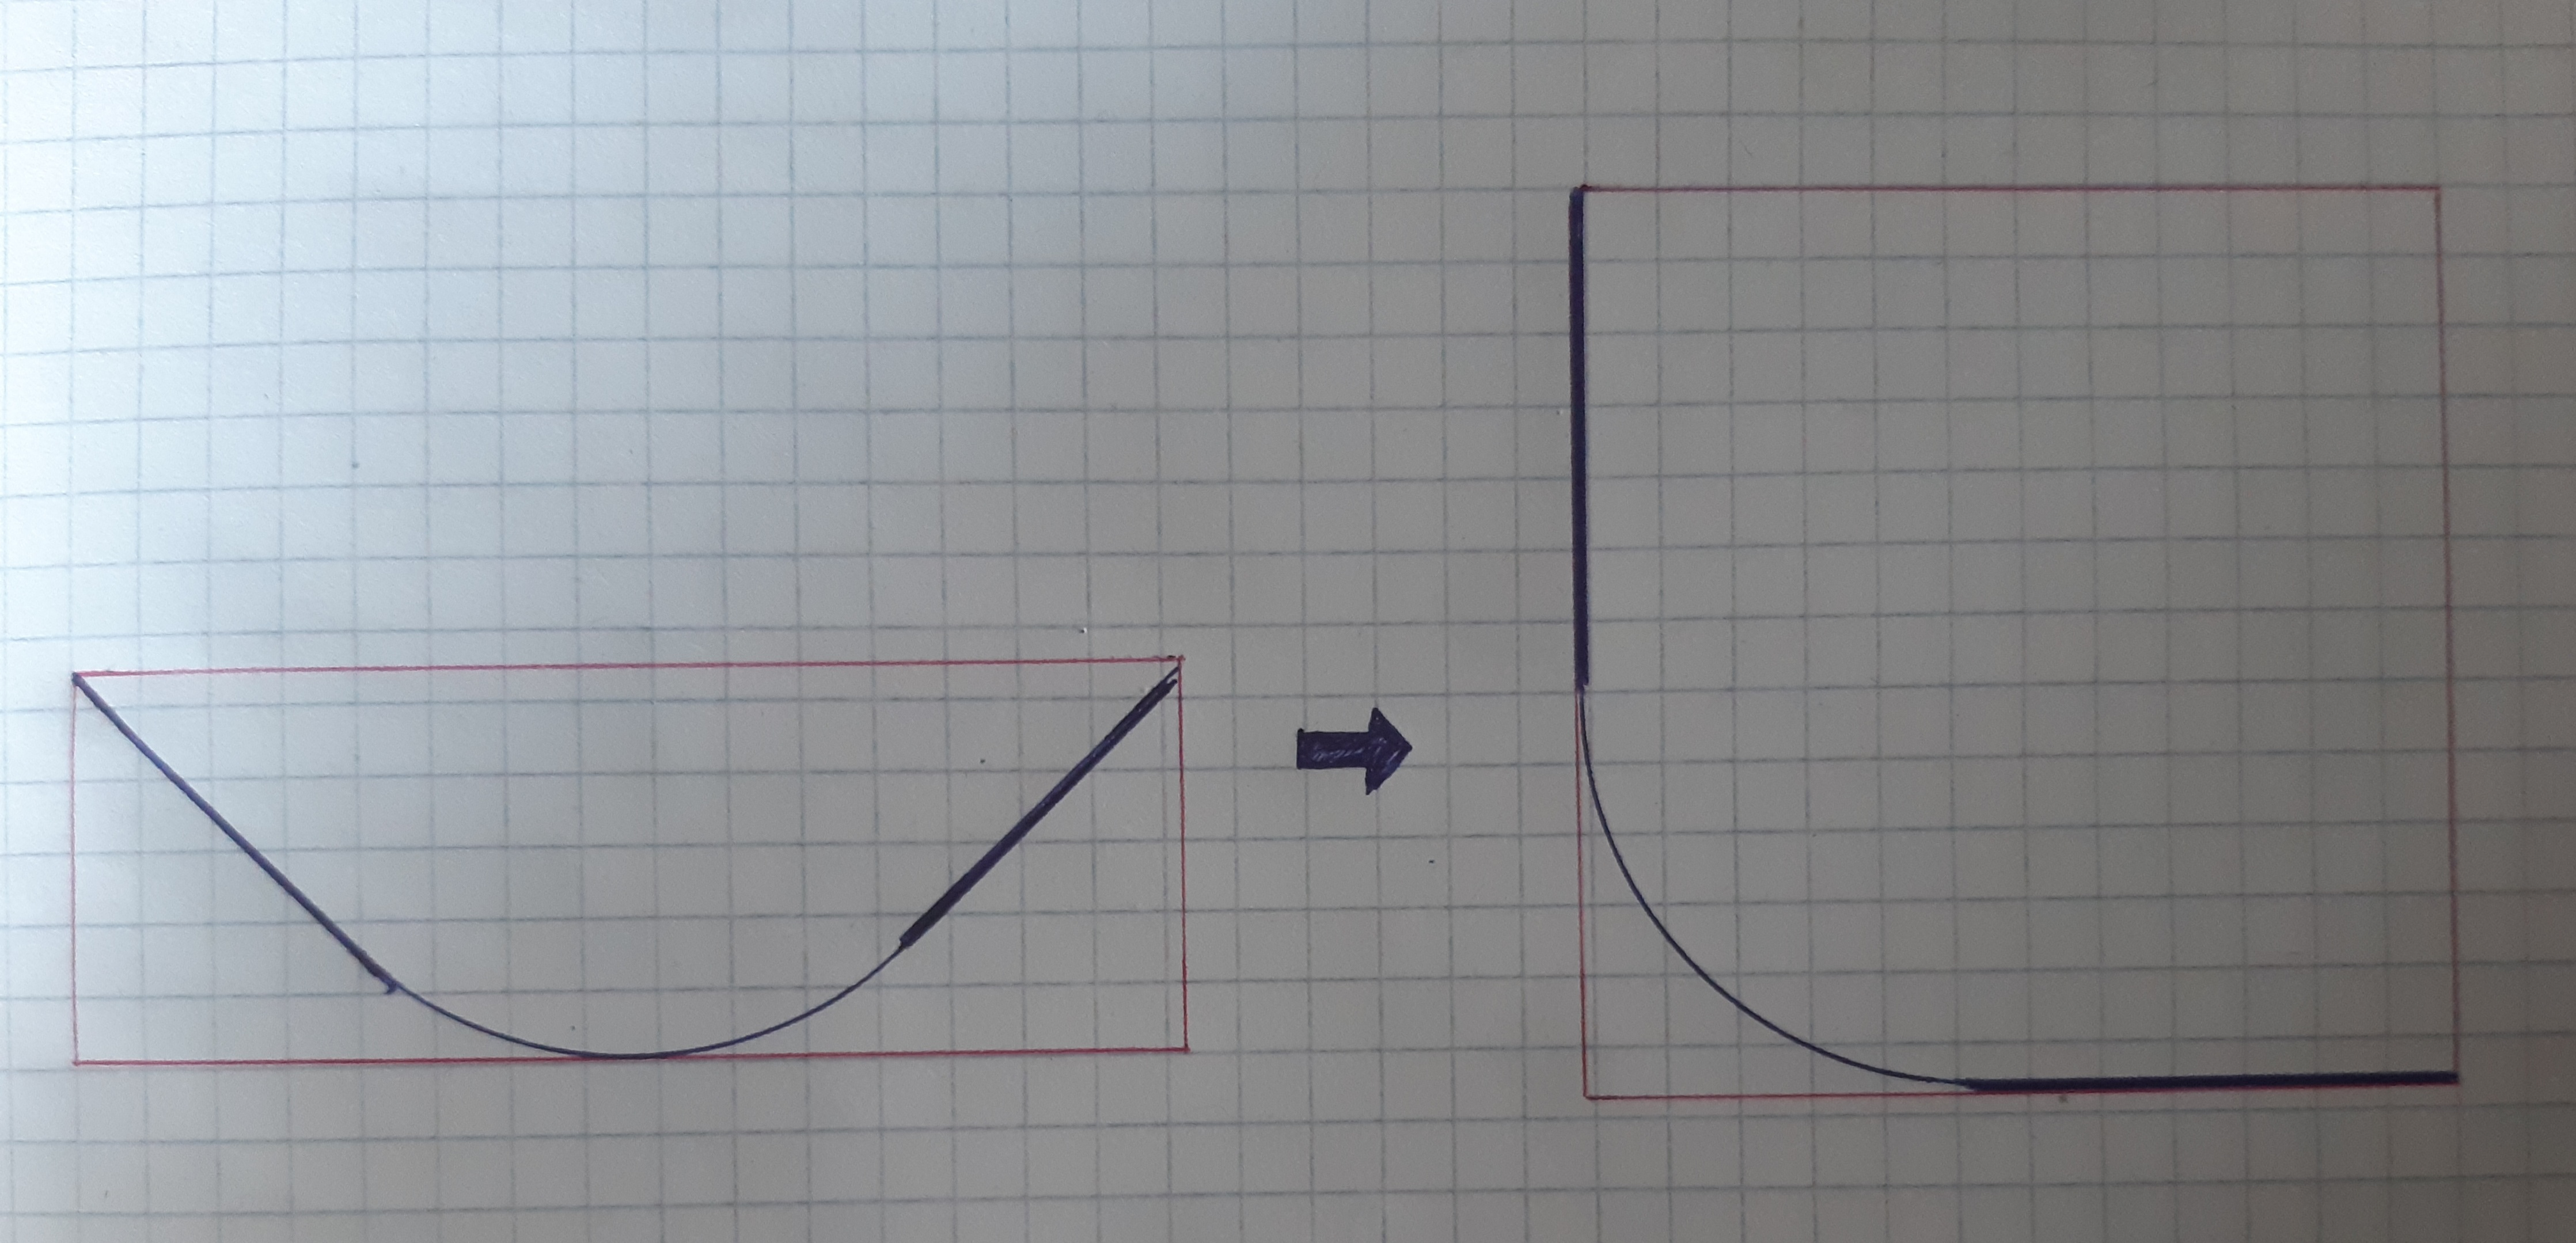
\includegraphics[height=5cm, width=9cm]{images/detect3.jpg}
     \captionof{figure}{Ротирање за $45^{\circ}$}
\end{center}
\vspace{0.5cm}
Слика десно се као аргумент прослијеђује функцији:
\begin{center}
\texttt{public static string detectBend2Rotated45(Mat img)}
\end{center}
у којој се врше све даље провјере. Са те слике се узимају одбирци по у-оси и проналази се регион одакле почиње закривљење. Затим се одсијеца регион на коме нема закривљења, а остатак слике се прослијеђује функцији \texttt{detectbend1FromHalf} тј. треба да задовољи све услове као лук класе 1. Ако задовољи, значи да је детестован лук облика L тј. лук класе 2.


\subsection{Провјера за класу 4 (састоји се од два L лука и заклапа $180^\circ$)}
\vspace{0.5cm}
\begin{center}
    \centering 
    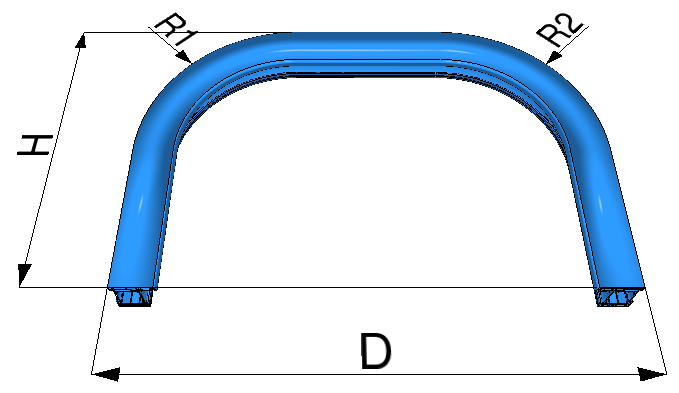
\includegraphics[height=4cm, width=6cm]{images/klasa4.jpg}
     \captionof{figure}{Класа 4}
\end{center}
\vspace{0.5cm}
За провјеру је задужена функција:
\begin{center}
\texttt{public static string detectBend4(Mat srcImg)}
\end{center}
из TimingScanner.bendClassifier класе.\\\\
Функција враћа стринг у коме су резултати провјере, а као параметap има:
\begin{itemize}
    \item \texttt{Mat srcImg} - улазна слика профила издвојена и ротирана тако да су краци профила окренути ка горе 
\end{itemize}
Логика за провјеру је следећа: Узме се само лијева половина слике и прослиједи се функцији detectBend2Rotated45 која је већ поменута горе. Половина лука класе 5 треба да буде лук класе 2, тј. лук облика L. Одатле логика коришћења претходне функције и у провјери за лук класе 5. Ако су резултати провјере позитивни, лук припада класи 5


\subsection{Провјера за класу 6 (вертикална елипса)}
\vspace{0.5cm}
\begin{center}
    \centering 
    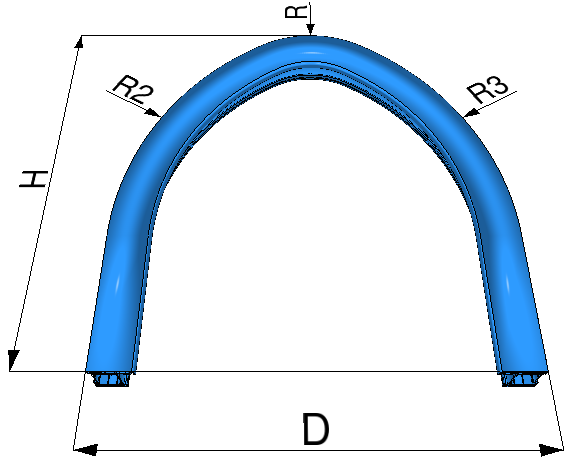
\includegraphics[height=4cm, width=6cm]{images/klasa6.jpg}
     \captionof{figure}{Класа 6}
\end{center}
\vspace{0.5cm}
За провјеру је задужена функција:
\begin{center}
\texttt{public static string detectBend6(Mat srcImg)}
\end{center}
из TimingScanner.bendClassifier класе.\\\\
Функција враћа стринг у коме су резултати провјере, а као параметap има:
\begin{itemize}
    \item \texttt{Mat srcImg} - улазна слика профила издвојена и ротирана тако да су краци профила окренути ка горе 
\end{itemize}
Логика је та да узмемо одбирке као и до сада, са лијеве стране ка десно. Од свих класа, лук ове класе има почетни одбирак са већом вриједношћу од половине ширине слике (лука) и на тај начин се врши провјера. Када се почетни одбирак и половина ширине пореде узима се и одређени проценат (p) за толеранцију тако да, ако вриједност првог одбирка означимо са h, вриједност половине ширине са w, тада треба да буде задовољено: h > w + p/100*w. Ако је тај услов задовољен, тада лук припада класи 6.



\subsection{Провјера за класу 3.1 (исјечак без равног дијела)}
\vspace{0.5cm}
\begin{center}
    \centering 
    
\includegraphics[height=1.7cm, width=6cm]{images/8_correct_rotation.png}
     \captionof{figure}{Класa 3.1 - исјечак без равног дијела}
\end{center}
\vspace{0.5cm}
За провјеру је задужена функција:
\begin{center}
\texttt{public static string isSectionWithoutFlat(Mat srcImg)}
\end{center}
из TimingScanner.bendClassifier класе.\\\\
Функција враћа стринг у коме су резултати провјере, а као параметap има:
\begin{itemize}
    \item \texttt{Mat srcImg} - улазна слика профила издвојена и ротирана тако да су краци профила окренути ка горе 
\end{itemize}
Ова класа лукова подразумјева само кружни исјечак без равног дијела а може да заклапа било који угао мањи од $180^\circ$ али без $180^\circ$ и без $90^\circ$ јер су та два заправо правилан и L лук за које смо већ имали провјеру и, с обзиром да те провјере нису прошле, одмах знамо да сигурно није кружни исјечак од $180^\circ$ или $90^\circ$. Ако претпоставимо да на слици јесте исјечак без равног дијела, тада ће свака тачка контуре бити тачка кружнице. Међутим, сада не знамо да претпоставимо дужину полупречника кружнице чији је исјечак дио. Оно што знамо јесу вриједности $a$ и $b$ са следеће слике, док се вриједност полупречника $r$ преко $a$ и $b$ рачуна по формули која је такође изведена на следећој слици:
\vspace{0.5cm}
\begin{center}
    \centering 
    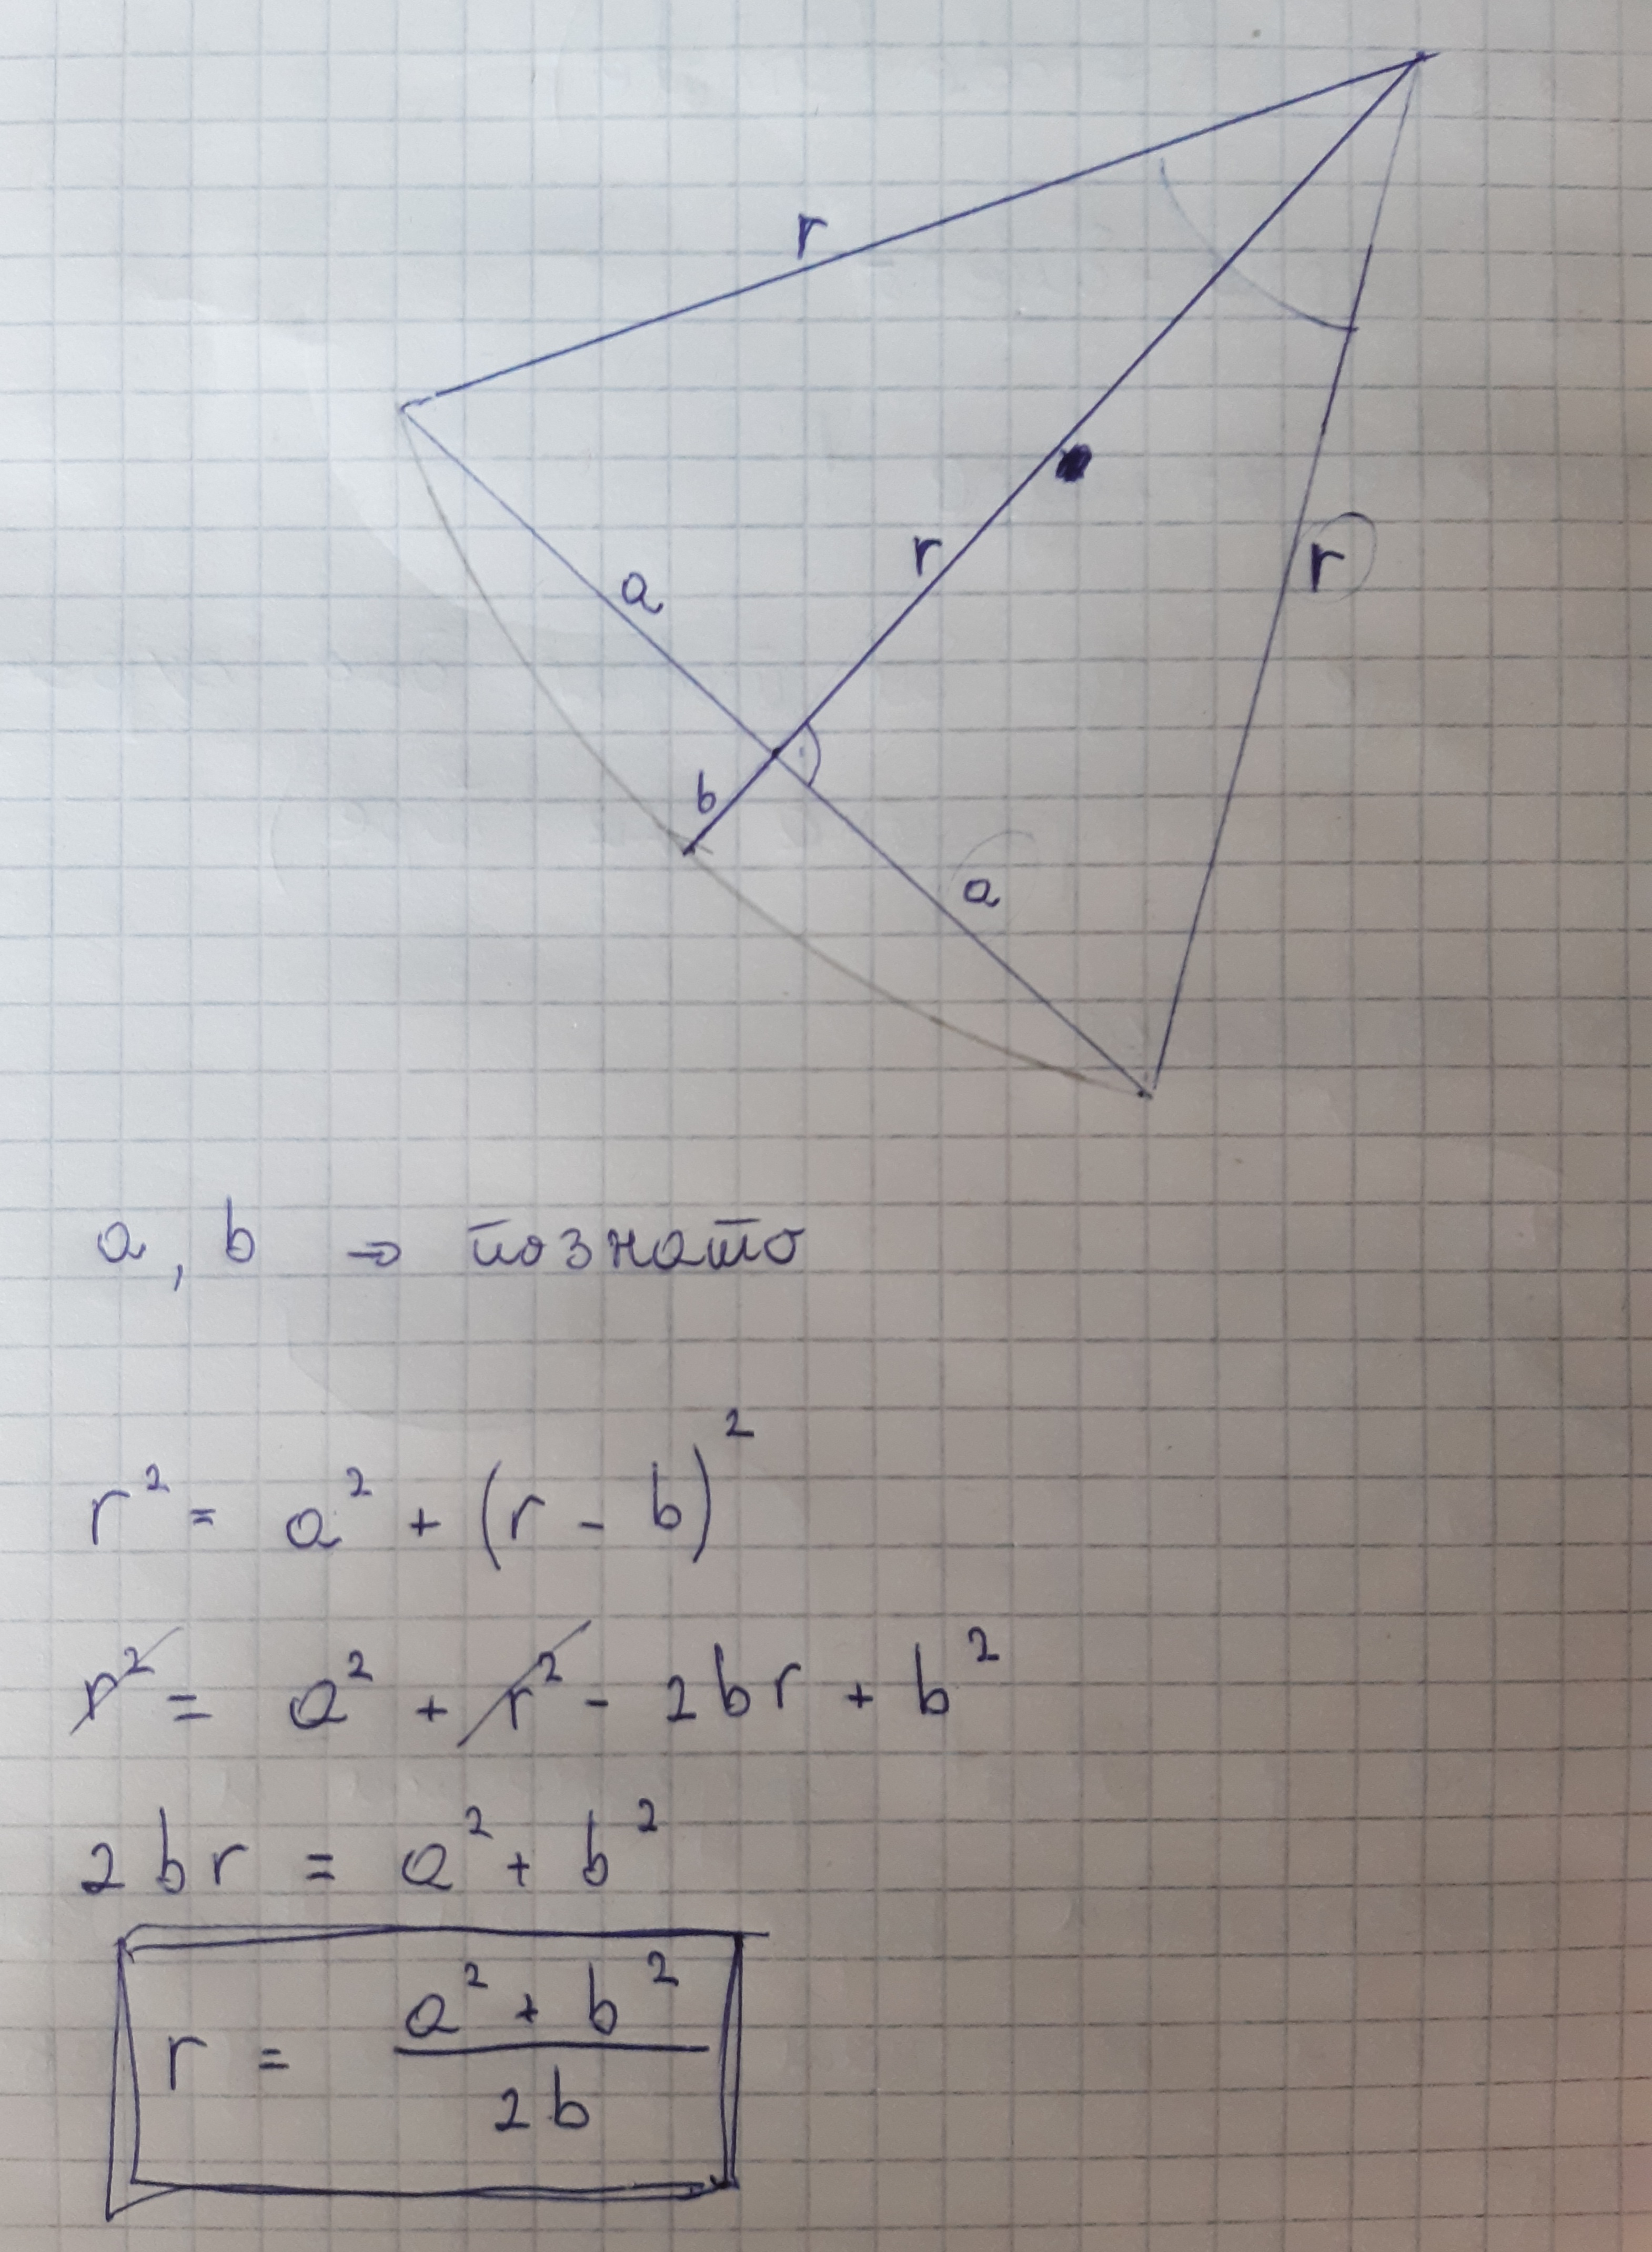
\includegraphics[height=12cm, width=10cm]{images/detect4.jpg}
     \captionof{figure}{Рачунање $r$ преко $a$ и $b$}
\end{center}
\vspace{0.5cm}


\subsection{Провјера за класе 3 (исјечак са равним дијелом) и 5 (хоризонтална елипса)}
\vspace{0.5cm}
\begin{center}
    \centering 
    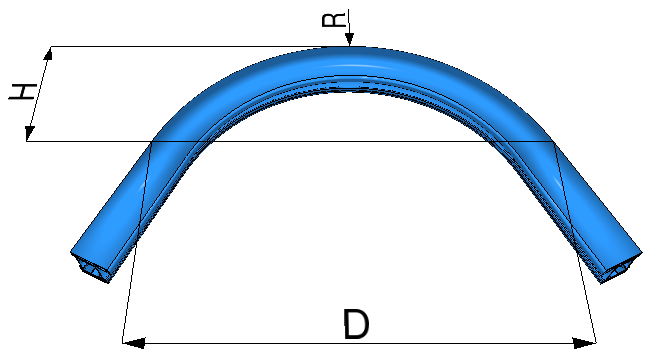
\includegraphics[height=4cm, width=6cm]{images/klasa3.jpg}
     \captionof{figure}{Класa 3}
\end{center}
\vspace{0.5cm}
\vspace{0.5cm}
\begin{center}
    \centering 
    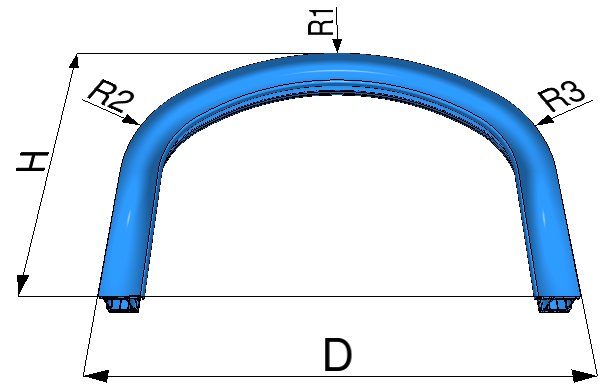
\includegraphics[height=4cm, width=6cm]{images/klasa5.jpg}
     \captionof{figure}{Класa 5}
\end{center}
\vspace{0.5cm}
За провјеру је задужена функција:
\begin{center}
\texttt{public static string detectBend3or5(Mat srcImg)}
\end{center}
из TimingScanner.bendClassifier класе.\\\\
Функција враћа стринг у коме су резултати провјере, а као параметap има:
\begin{itemize}
    \item \texttt{Mat srcImg} - улазна слика профила издвојена и ротирана тако да су краци профила окренути ка горе 
\end{itemize}
С обзиром да провјере до ове нису прошле остаје могућност да су на слици или исјечак са продужетком (класа 3) или хоризонтална елипса (класа 5). То значи да је потребно пронаћи кључну разлику између њих. Та разлика је у равном дијелу којим почиње лук класе 3, насупрот луку класе 5 који на истом дијелу мора имати неко закривљење. Тај дио је приказан на следећој слици заокружен зеленом бојом:
\vspace{0.5cm}
\begin{center}
    \centering 
    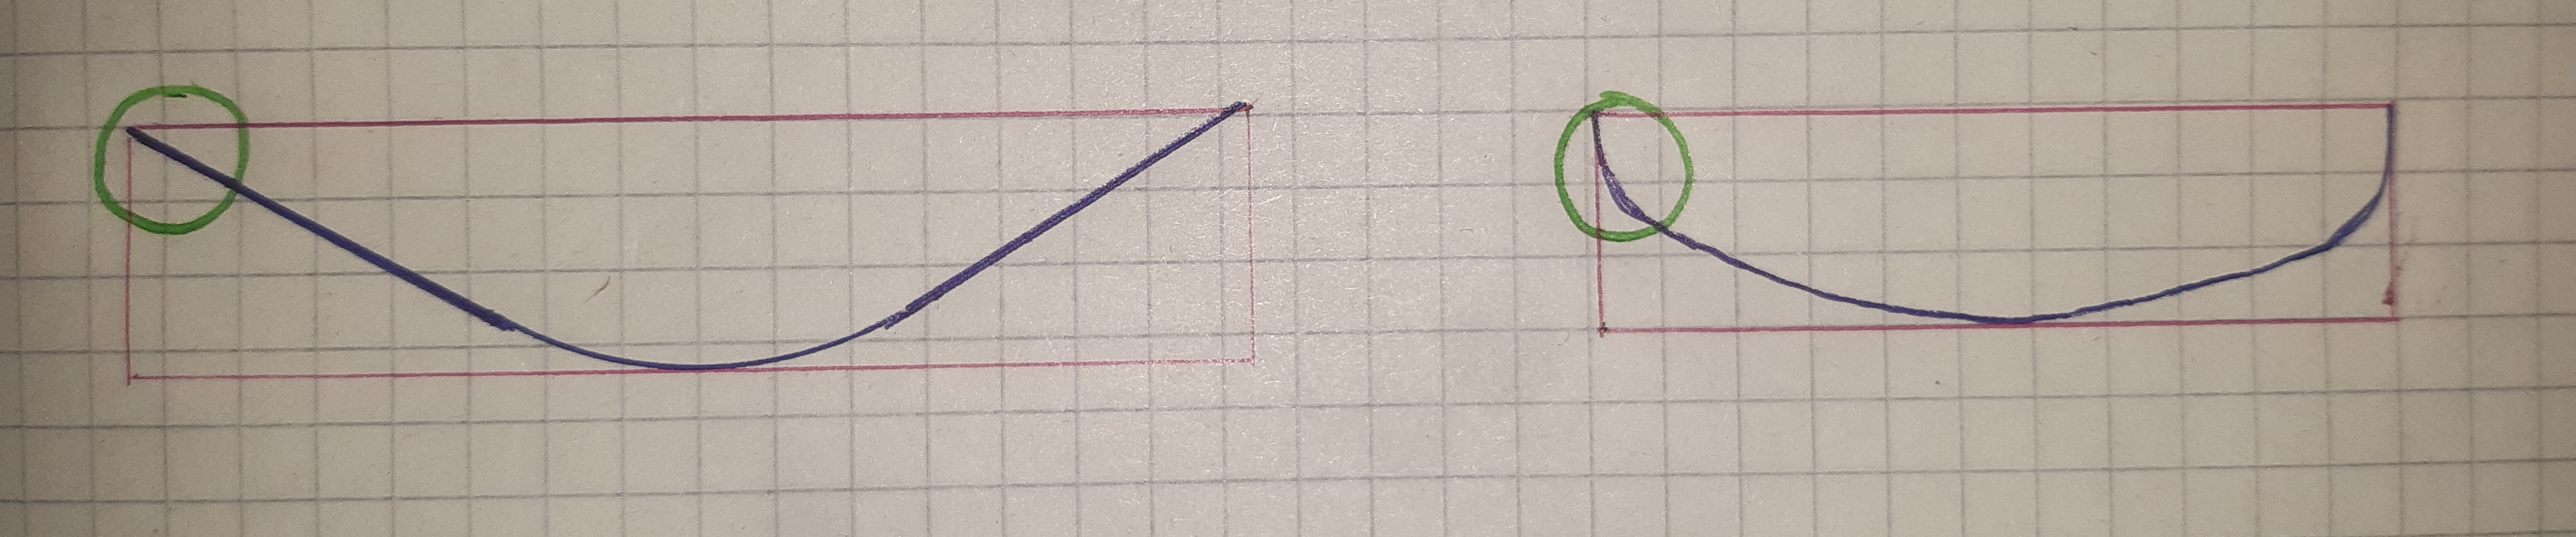
\includegraphics[height=4cm, width=15cm]{images/detect5.jpg}
     \captionof{figure}{Разлика између класе 3 (лијево) и класе 5 (десно)}
\end{center}
\vspace{0.5cm}
Одабир је имплементиран тако да се узима 1/5 лијеве половине улазне слике профила и узму се усредњене вриједности одбирака за тај дио. Кроз први и последњи одбирак се провуче права и одреде њени коефицијенти $k$ и $n$. Након тога пролазимо кроз све остале тачке између, и ако постоји одступање од праве које је веће од неког предвиђеног одступања, то значи да тај дио није раван и да је лук класе 5 тј. вертикална елипса. Ако је дио детектован као раван, тада је лук класе 3 тј. исјечак без продужетка који заклапа мање од $180^\circ$ али без $90^\circ$



\newpage
\section{Закључак}
Као закључак је потребно навести потенцијална побољшања класификатора, као и могућности које добро направљен класификатор даје за даљи развој. Све функционалности урађеног класификатора потребно је још много тестирати и радити на њиховом побољшању. У оквиру овог пројекта претпостављала су се нека ограничења која иначе не морају да постоје. Нека од њих су: увијек иста удаљеност профила од камере, не узимање у обзир перспективе у току издвајања профила, краци профила су увијек исте дужине итд. Нпр профил не мора да има краке исте дужине и може да изгледа као на следећој слици:
\vspace{0.5cm}
\begin{center}
    \centering 
    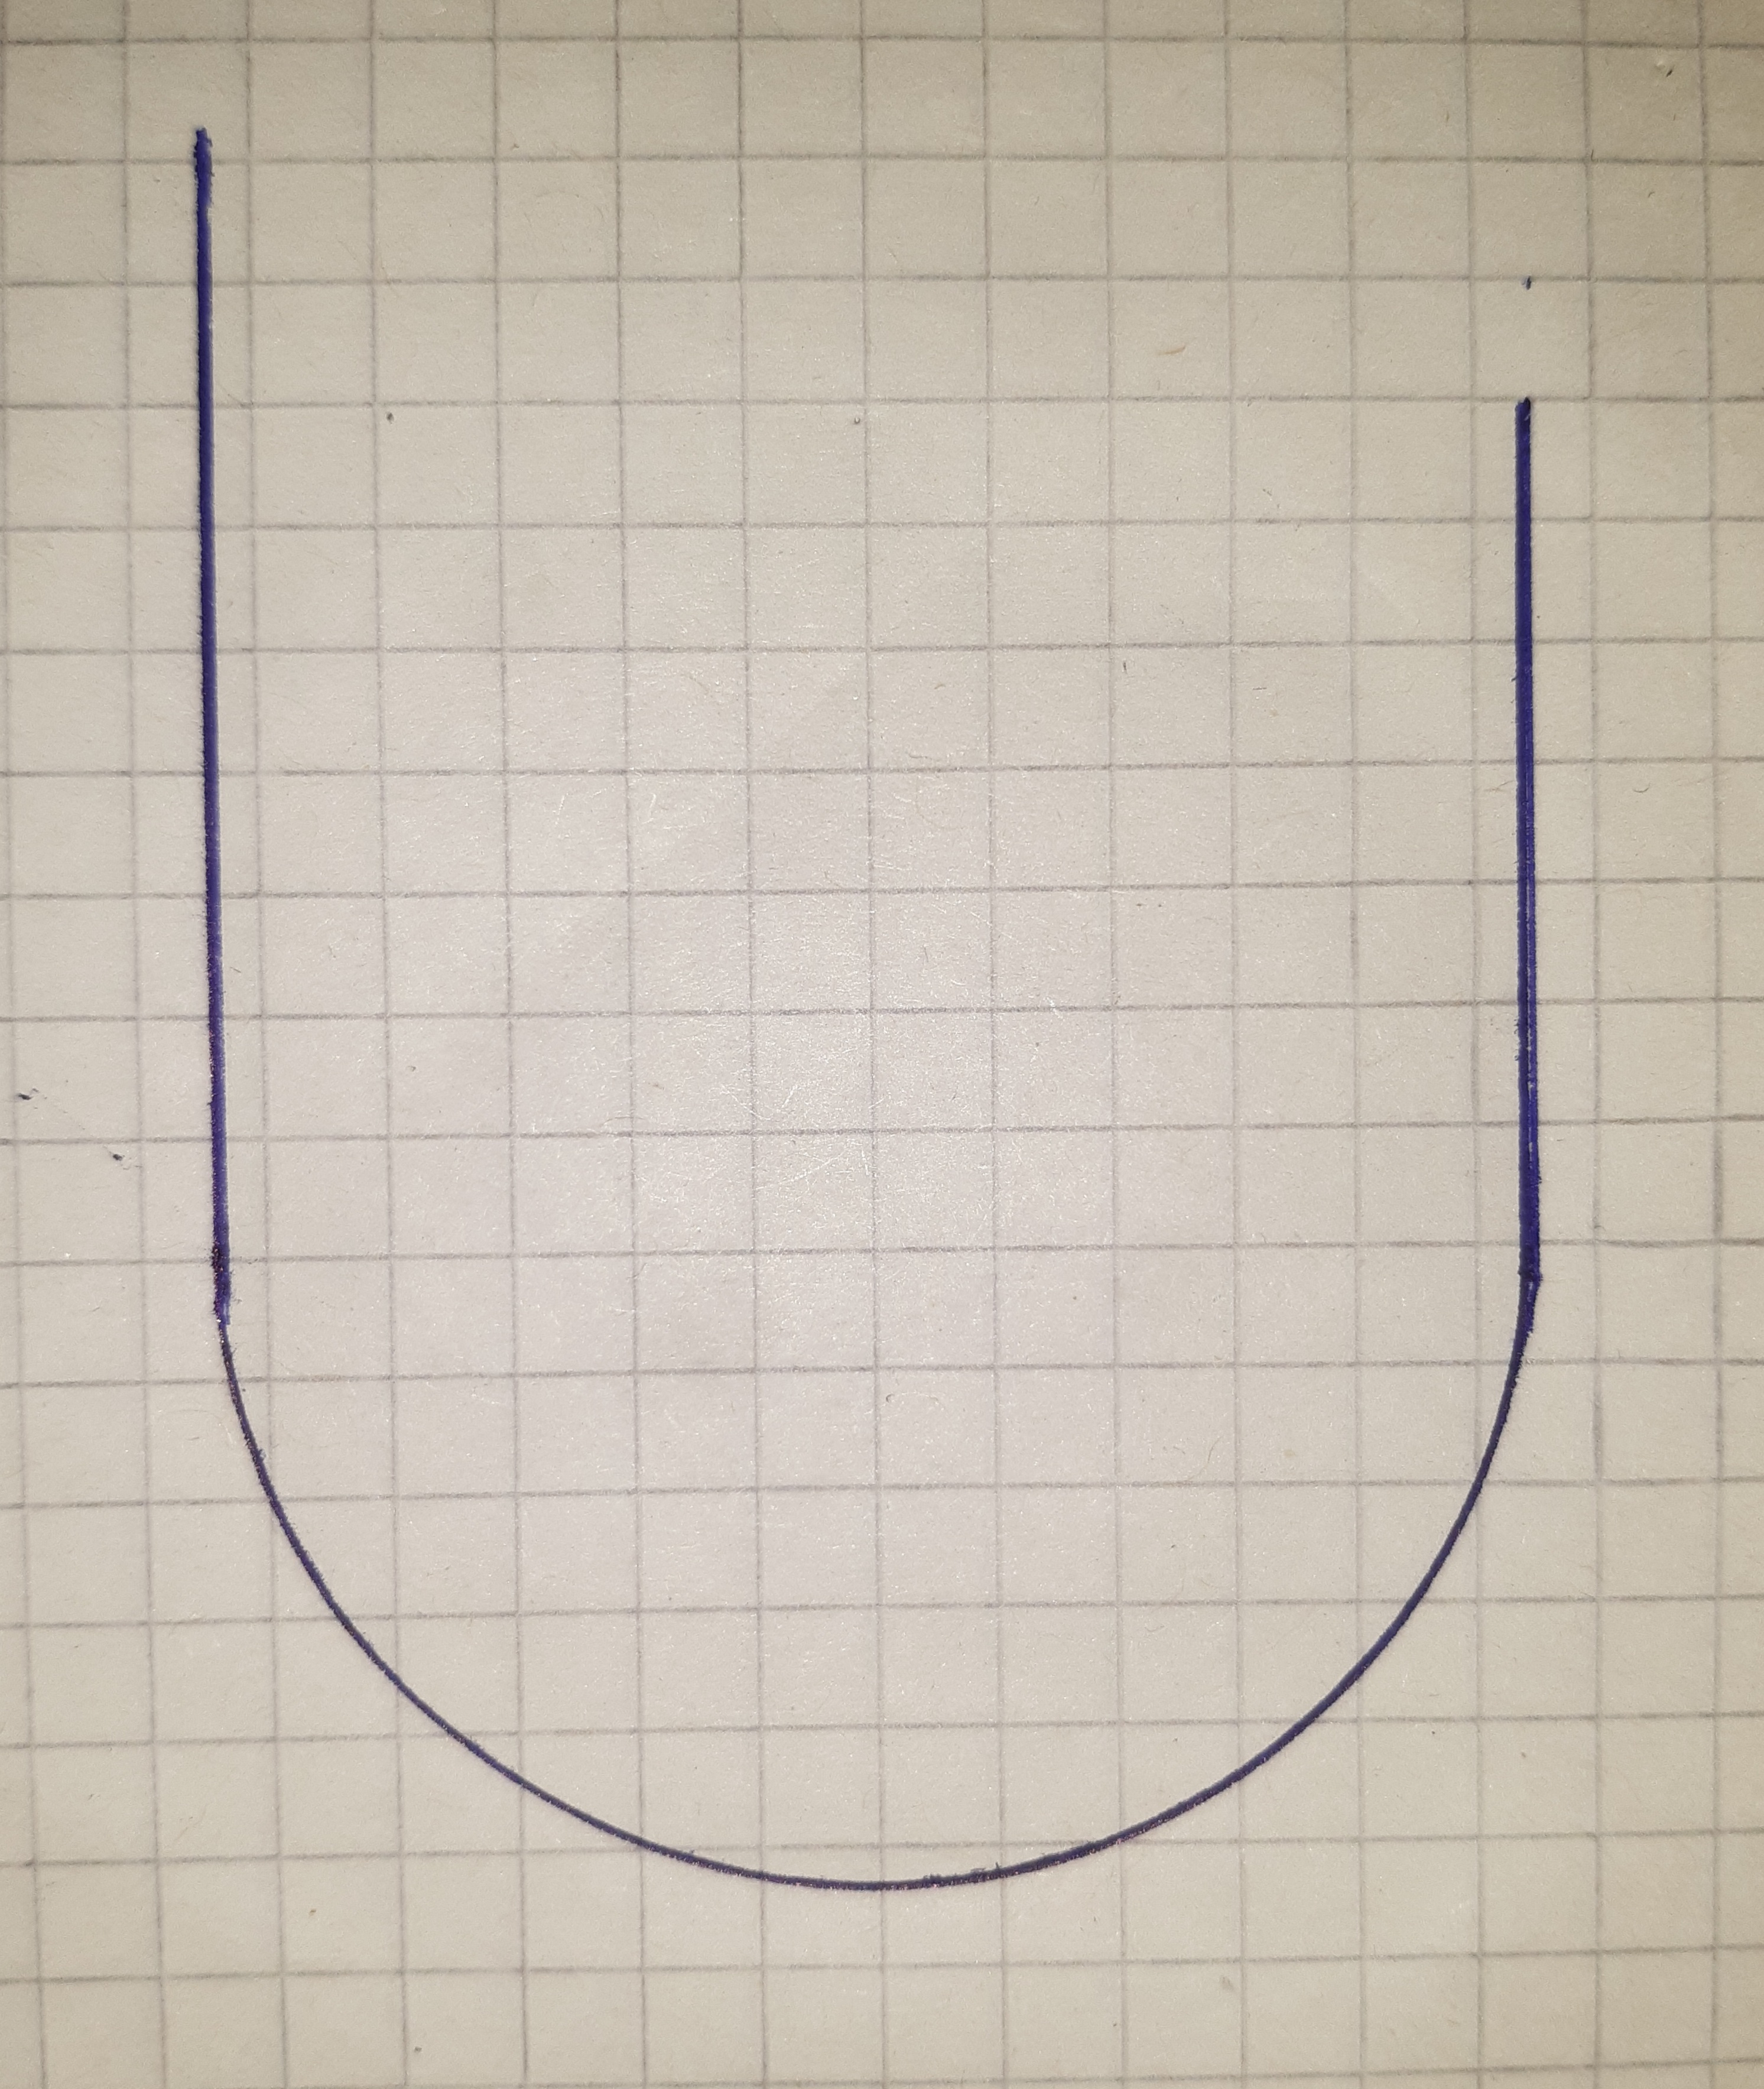
\includegraphics[height=6cm, width=5cm]{images/zakljucak1.jpg}
     \captionof{figure}{Изглед профила чији су краци неједнаке дужине}
\end{center}
\vspace{0.5cm}
У претходном случају, ако треба да се изврши корекција ротације, неће радити баш тако као над профилима једнаких крака. Због таквих и сличних ситуација које нису узете у обзир намеће се потреба за следећим побољшањима:
\begin{itemize}
    \item Прецизније отклањање шума
    \item Отклањање равног дијела било које контуре тако да остане само лук (веома пожељна функционалност која није баш тривијална за имплементацију поготово ако не знамо ништа о томе како је профил окренут)
    \item Прецизније усредњавање одбирака (нпр. ако се очекује да је сваки одбирак мањи од претходног, тада умјесто замјене тог одбирка са просјечном вриједношћу претходног и наредног, одбирак мијењамо са претходним, јер тако правимо, у том моменту, минималну грешку)
\end{itemize}
Након успјешне имплементације класификатора, скенер се у будућности може надоградити на функционалности мјерења углова закривљености профила.

\newpage
\section{Литература}
\begin{itemize}
  \item \url{https://www.coursera.org/specializations/deep-learning}
  \item \url{https://elektrotehnika.github.io/dl/}
  \item \url{https://www.overleaf.com/project}
  \item \url{https://shimat.github.io/opencvsharp_docs/html/d69c29a1-7fb1-4f78-82e9-79be971c3d03.htm}
  \item \url{https://docs.opencv.org/4.x/index.html}
  \item \url{https://docs.opencv.org/3.4/db/df6/tutorial_erosion_dilatation.html}
  \item \url{https://stackoverflow.com/}
\end{itemize}

\end{document}
